\section{Clasificación}%\label{sec:clasificacion}
La clasificación automática de textos según su nivel de dificultad lingüística constituye un componente central en múltiples escenarios educativos, especialmente en aquellos vinculados a la enseñanza de lenguas extranjeras. En este trabajo nos centramos en la tarea de asignar niveles del CEFR a textos en inglés, con el objetivo de automatizar la selección de materiales adecuados para distintos perfiles de estudiantes. Esta tarea resulta esencial en entornos donde se manejan grandes volúmenes de contenido educativo, y donde la escalabilidad, consistencia y adaptabilidad son requisitos fundamentales.

Históricamente, la clasificación de dificultad textual se basó en enfoques estáticos construidos sobre características predefinidas: longitud de las oraciones, complejidad léxica, frecuencia de vocabulario, estructuras gramaticales recurrentes y otros indicadores superficiales de legibilidad. Si bien estos métodos han proporcionado resultados razonables en contextos específicos, presentan limitaciones importantes: requieren una intensa ingeniería de características, dependen de corpus anotados de alta calidad y son poco tolerantes a variaciones de estilo, dominio o género textual.

Con el surgimiento de los LLMs, se abre la posibilidad de adoptar estrategias más flexibles, capaces de capturar patrones semánticos, sintácticos y discursivos sin necesidad de diseñar manualmente los rasgos relevantes. En este capítulo analizamos el rendimiento de distintos LLMs open-source y privativos en la clasificación CEFR, empleando estrategias livianas basadas en prompting, incluyendo prompts pedagógicos, descriptores CEFR, ejemplos seleccionados por docentes expertos y, cuando es relevante, técnicas de “conocimiento de dominio” incorporado mediante instrucciones estructuradas. Estas aproximaciones permiten explorar el conocimiento lingüístico latente en los modelos sin recurrir necesariamente a entrenamiento adicional.

No obstante, dado que los LLMs no siempre alcanzan niveles de precisión suficientes mediante prompting, integramos también una etapa de fine-tuning específica para la tarea. A través de este proceso, buscamos evaluar hasta qué punto la adaptación supervisada de un modelo preentrenado mejora su capacidad para discriminar niveles cercanos y estabiliza su comportamiento ante variaciones en la longitud o estructura del prompt.

La sección se organiza de la siguiente manera. En primer lugar, revisamos la literatura existente en evaluación de legibilidad, clasificación CEFR y aplicaciones de LLMs en educación (\Cref{subsection:clas_trabajo}). Luego describimos los experimentos diseñados (\Cref{subsection:clas_diseño}), los prompts utilizados (\Cref{subsection:clas_prompt}), las métricas empleadas (\Cref{subsection:clas_metrica}), el proceso de fine-tuning (\Cref{subsection:clas_finetuning}) y, finalmente, presentamos un análisis detallado de los resultados (\Cref{subsection:clas_resuslt}), discusión (\Cref{subsection:clas_discusion}), conclusiones (\Cref{subsection:clas_conclusiones}) y trabajo futuro (\Cref{subsection:clas_trab_fut}).

\subsection{Trabajo relacionado}\label{subsection:clas_trabajo}
La clasificación automática según niveles del CEFR se sitúa en la intersección de tres campos de investigación: la evaluación automática de legibilidad (ARA), la clasificación de textos en PLN y los enfoques específicos desarrollados para la predicción de niveles lingüísticos. En esta sección sintetizamos las principales contribuciones de cada área para contextualizar los enfoques adoptados en este trabajo.

\subsubsection*{Evaluación automática de legibilidad (ARA)}
La Automatic Readability Assessment (ARA) se ocupa de modelar la dificultad de lectura y comprensión de un texto para una audiencia determinada. Los primeros enfoques se basaron en fórmulas de legibilidad tradicionales, como Flesch-Kincaid \parencite{Kincaid1975} o SMOG \parencite{smog}, que describen la complejidad textual a partir de indicadores superficiales (longitud de palabras, sílabas, longitud de oraciones). Aunque estas métricas han sido ampliamente utilizadas por su simplicidad y bajo costo computacional, resultan insuficientes para capturar aspectos más profundos del lenguaje, como la coherencia discursiva o la complejidad sintáctica.

A partir de los años 2000, el campo incorporó técnicas de PLN que permiten modelar de manera más rica los fenómenos lingüísticos involucrados en la legibilidad. Se exploraron características léxicas (riqueza, diversidad), morfológicas, sintácticas (profundidad de árbol, ambigüedad), discursivas (marcadores, relaciones retóricas), así como representaciones distribucionales basadas en embeddings. Estas aproximaciones mejoraron significativamente la precisión en contextos para hablantes nativos y, posteriormente, comenzaron a adaptarse para aprendices L2, un avance especialmente relevante para CEFR.

La evaluación para L2 presenta desafíos propios: el vocabulario disponible para un aprendiz crece de manera incremental, la gramática internalizada se desarrolla heterogéneamente y la familiaridad con distintos géneros textuales varía ampliamente. En consecuencia, las herramientas diseñadas para hablantes nativos no siempre se trasladan adecuadamente a contextos educativos de lengua extranjera. Esto motivó el desarrollo de sistemas especializados, muchos de ellos adoptados por plataformas educativas y pruebas estandarizadas.

\subsubsection*{Clasificación de textos en PLN}
La clasificación de textos es una de las tareas más estudiadas del PLN. Los enfoques clásicos basados en bag-of-words o n-grams han sido progresivamente desplazados por arquitecturas profundas, especialmente CNNs, RNNs y transformers. La aparición de modelos preentrenados a gran escala, como BERT, RoBERTa o GPT, transformó por completo la manera de abordar esta tarea, desplazando la ingeniería de características hacia estrategias basadas en transferencia de conocimiento \parencite{Zhou2020, Li2021, benchmark}.

Los estudios de revisión coinciden en que los transformers superan sistemáticamente a los métodos tradicionales, tanto en precisión como en estabilidad, incluso en escenarios con datos limitados. Esto es especialmente relevante para CEFR, donde la disponibilidad de corpus no siempre es uniforme y donde las fronteras entre clases adyacentes pueden resultar difusas incluso para anotadores humanos \parencite{Kerz2021, Wisniewski2017}.

\subsubsection*{Clasificación CEFR con machine learning y LLMs}

La investigación orientada específicamente a predecir niveles CEFR ha seguido una evolución coherente con el desarrollo de las técnicas de PLN:

\begin{itemize}
    \item \textbf{Modelos clásicos con features manuales}
    
    Enfoques iniciales combinaron características estilísticas, léxicas y sintácticas con algoritmos como SVMs o regresión logística \parencite{Xia2019}. Aunque efectivos, su rendimiento se veía limitado por la necesidad de diseñar cuidadosamente los rasgos y por su baja capacidad de generalización.

    \item \textbf{Transformers ajustados a corpus CEFR}
    Con la llegada de modelos como BERT, los F1-scores mejoraron notablemente. Estos avances mostraron que las representaciones profundas capturan diferencias lingüísticas más sutiles que los enfoques basados en reglas \parencite{JulianaSchmalz2021}.

    \item \textbf{Herramientas especializadas}
    Sistemas como el EDIA CEFR Tagger \parencite{edia}, Text Inspector \parencite{text_inspector} o Cathoven \parencite{cathoven} que integran modelos clasicos con recursos lingüísticos interpretables, aunque ultimamente tambien implementan modelos neuronales o LLMs. Su uso se ha extendido en contextos educativos, aunque generalmente operan como cajas cerradas.

    \item \textbf{LLMs y prompting}
    Investigaciones recientes han explorado hasta qué punto los LLMs internalizan el conocimiento de la escala CEFR y son capaces de replicar el juicio de un evaluador experto. Trabajos como el de \parencite{Benedetto2025} evalúan esta capacidad mediante una suite de tareas diseñadas para medir si los modelos han codificado adecuadamente los requisitos pedagógicos del marco, utilizando técnicas de prompting que van desde el zero-shot hasta enfoques orientados al razonamiento. Por otro lado, estudios centrados en idiomas específicos, como el de \parencite{aleman} para el alemán, demuestran que si bien el prompt engineering ofrece resultados prometedores, el fine-tuning de modelos como Llama-3-8B permite alcanzar niveles de precisión superiores. No obstante, los resultados globales siguen siendo dispares: aunque los modelos logran distinguir diferencias amplias entre niveles (ej. A1 vs. C2), persiste una dificultad significativa para clasificar niveles adyacentes, especialmente en la transición B1–B2 y B2–C1, donde las fronteras de los descriptores cualitativos suelen solaparse.

    \item \textbf{Corpus multilingües y estudios comparativos}
    La publicación de datasets como UniversalCEFR \parencite{Imperial2025} habilitó investigaciones que exploran transfer learning entre lenguas, demostrando que los LLMs pueden beneficiarse de similitudes estructurales entre idiomas.
\end{itemize}

En conclusión, el análisis del trabajo relacionado expone que, si bien los LLMs representan la frontera actual en la clasificación CEFR, las investigaciones vigentes oscilan entre el diseño de instrucciones y el ajuste fino de modelos particulares sin alcanzar un estándar definitivo, persistiendo la dificultad para diferenciar niveles contiguos. Ante este escenario, la propuesta de esta investigación se centra en abordar dicha brecha mediante una evaluación sistemática y comparativa de múltiples modelos de código abierto bajo diferentes estrategias de prompting. En lugar de restringir el análisis a una única solución, este estudio explora de manera exhaustiva la interacción entre diversas arquitecturas y estructuras de instrucciones.

\subsection{Diseño de Experimentos}\label{subsection:clas_diseño}
El objetivo de esta sección es describir de manera sistemática el diseño experimental utilizado para evaluar las capacidades de distintos modelos de lenguaje en la clasificación de textos según los niveles del CEFR. La organización de los experimentos se estructuró en torno a tres dimensiones principales: (i) la comparación entre modelos, (ii) la evaluación de diferentes estrategias de prompting, y (iii) la exploración del impacto de conocimiento lingüístico explícito mediante instrucciones o ejemplos seleccionados. A continuación se detallan estas dimensiones.

\subsubsection*{Selección de modelos}
Se evaluaron tanto modelos open-source como propietarios, con el fin de obtener una perspectiva amplia del estado del arte. Entre los modelos abiertos se incluyeron representantes de las familias LLaMA, Mistral y Gemma, seleccionados por su disponibilidad pública, su rango de tamaños y su relevancia en aplicaciones educativas. Además, incorporamos ChatGPT y DeepSeek como referencia del rendimiento alcanzable con sistemas privativos ampliamente utilizados en entornos no académicos.

Es importante señalar que, en el caso de los modelos propietarios como Chat GPT y DeepSeek, se accedió a su servicio a través de una API Key.
Por motivos de costo y políticas de acceso, los modelos propietarios solo pudieron utilizarse en una fracción de los experimentos. Su inclusión no persiguió integrar estas herramientas en un flujo de trabajo reproducible, sino obtener una referencia comparativa respecto de soluciones altamente optimizadas pero cerradas.

Por otro lado, incorporamos herramientas especializadas en análisis de dificultad textual, como Text Inspector, Cathoven y el clasificador del TSAR, utilizadas como referencias simbólicas off-the-shelf del estado del arte. Esta doble estrategia nos permitió contrastar las capacidades de los LLMs con aproximaciones tradicionales diseñadas específicamente para esta tarea.

\subsection{Modalidades de prompting}\label{subsection:clas_prompt}
Ademas de los modelos, se decidio comparar distintas estrategias de prompting que buscan orientar al modelo desde aproximaciones con prompt simples, hasta variantes que incorporan conocimiento lingüístico explícito o ejemplos representativos.

Se definieron tres grandes grupos:
\begin{itemize}
    \item \textbf{Prompting directo (0-shot)}
    El modelo recibe únicamente el texto a clasificar y una instrucción breve que solicita la asignación de un nivel CEFR.

    \item \textbf{Prompting con conocimiento de dominio}
    Se añadieron elementos derivados de prácticas docentes de enseñanza de inglés como L2, como descriptores de nivel CEFR o listas de palabras por nivel.

    \item \textbf{Prompting con ejemplos (1-shot y 2-shot)}
    Los ejemplos fueron seleccionados por docentes expertos de manera cuidadosa. Se proporcionaron textos con su nivel CEFR correspondiente, con el fin de suministrar patrones lingüísticos representativos.
\end{itemize}

En todos los grupos, también se evaluó la influencia del sesgo de sobre-clasificación en B2 (descubierta en etapas tempranas del proyecto) y como mitigar esto, diseñando prompts que excluían explícitamente dicho nivel o que se le indicaba al modelo del problema y se le pedia que lo corrigiera. Además, se evaluó la diferencia entre la clasificacion dada si se pide que sea para una tarea de lecto comprensión o no.

Esto dio lugar a un conjunto amplio de prompts, enumerados y resumidos posteriormente en la Tabla \ref{tab:resumen_prompts}, ademas en el \Cref{sec:prompts} se encuentran en mas detalle cada prompt. Luego, cada experimento corresponde a la combinación de un modelo y un prompt, asegurando la comparabilidad entre modelos y estrategias.

\begin{landscape}
\begin{table}[p]
\resizebox{\linewidth}{!}{%
\begin{tabular}{@{}clllllllll@{}}
\toprule
\textbf{número} &
  \multicolumn{1}{c}{\textbf{0-shot}} &
  \multicolumn{1}{c}{\textbf{1-shot}} &
  \multicolumn{1}{c}{\textbf{2-shot}} &
  \multicolumn{1}{c}{\makecell{\textbf{con lecto}\\\textbf{comprensión}}} &
  \multicolumn{1}{c}{\makecell{\textbf{criterios}\\\textbf{pedagógicos}}} &
  \multicolumn{1}{c}{\makecell{\textbf{corrección}\\\textbf{de sesgo}}} &
  \multicolumn{1}{c}{\makecell{\textbf{eliminación de}\\\textbf{referencias B2}}} &
  \multicolumn{1}{c}{\makecell{\textbf{descriptores}\\\textbf{de nivel}}} &
  \multicolumn{1}{c}{\makecell{\textbf{palabras}\\\textbf{por nivel}}} \\ \midrule
0 &
  \multicolumn{1}{c}{x} &
   &
   &
   &
   &
   &
   &
   &
   \\
1 &
  \multicolumn{1}{c}{x} &
   &
   &
  \multicolumn{1}{c}{x} &
   &
   &
   &
   &
   \\
2 &
  \multicolumn{1}{c}{x} &
   &
   &
   &
   &
  \multicolumn{1}{c}{x} &
   &
   &
   \\
3 &
  \multicolumn{1}{c}{x} &
   &
   &
  \multicolumn{1}{c}{x} &
   &
  \multicolumn{1}{c}{x} &
   &
   &
   \\
4 &
  \multicolumn{1}{c}{x} &
   &
   &
   &
  \multicolumn{1}{c}{x} &
   &
   &
   &
   \\
5 &
  \multicolumn{1}{c}{x} &
   &
   &
   &
  \multicolumn{1}{c}{x} &
   &
   &
   &
   \\
6 &
  \multicolumn{1}{c}{x} &
   &
   &
   &
  \multicolumn{1}{c}{x} &
   &
   &
   &
   \\
7 &
  \multicolumn{1}{c}{x} &
   &
   &
   &
  \multicolumn{1}{c}{x} &
   &
   &
   &
   \\
8 &
  \multicolumn{1}{c}{x} &
   &
   &
   &
  \multicolumn{1}{c}{x} &
   &
   &
   &
   \\
9 &
   &
  \multicolumn{1}{c}{x} &
   &
   &
   &
   &
   &
   &
   \\
10 &
   &
  \multicolumn{1}{c}{x} &
   &
  \multicolumn{1}{c}{x} &
   &
   &
   &
   &
   \\
11 &
   &
  \multicolumn{1}{c}{x} &
   &
   &
   &
  \multicolumn{1}{c}{x} &
   &
   &
   \\
12 &
   &
  \multicolumn{1}{c}{x} &
   &
  \multicolumn{1}{c}{x} &
   &
  \multicolumn{1}{c}{x} &
   &
   &
   \\
13 &
   &
  \multicolumn{1}{c}{x} &
   &
   &
   &
   &
  \multicolumn{1}{c}{x} &
   &
   \\
14 &
   &
  \multicolumn{1}{c}{x} &
   &
  \multicolumn{1}{c}{x} &
   &
   &
  \multicolumn{1}{c}{x} &
   &
   \\
15 &
   &
   &
  \multicolumn{1}{c}{x} &
   &
   &
   &
   &
   &
   \\
16 &
   &
   &
  \multicolumn{1}{c}{x} &
  \multicolumn{1}{c}{x} &
   &
   &
   &
   &
   \\
17 &
   &
   &
  \multicolumn{1}{c}{x} &
   &
   &
  \multicolumn{1}{c}{x} &
   &
   &
   \\
18 &
   &
   &
  \multicolumn{1}{c}{x} &
  \multicolumn{1}{c}{x} &
   &
  \multicolumn{1}{c}{x} &
   &
   &
   \\
19 &
   &
   &
  \multicolumn{1}{c}{x} &
   &
   &
   &
  \multicolumn{1}{c}{x} &
   &
   \\
20 &
   &
   &
  \multicolumn{1}{c}{x} &
  \multicolumn{1}{c}{x} &
   &
   &
  \multicolumn{1}{c}{x} &
   &
   \\
21 &
   &
   &
   &
   &
   &
   &
   &
  \multicolumn{1}{c}{x} &
   \\
22 &
   &
   &
   &
   &
   &
   &
  \multicolumn{1}{c}{x} &
  \multicolumn{1}{c}{x} &
   \\
23 &
   &
   &
   &
   &
   &
   &
   &
   &
  \multicolumn{1}{c}{x} \\ \bottomrule
\end{tabular}}
\caption{Resumen de las características lingüísticas y de prompting que tiene cada prompt.}
\label{tab:resumen_prompts}
\end{table}
\end{landscape}

Las diferentes aproximaciones para crear prompts producen largos de prompt también muy diferentes. Como se puede observar en la Figura \ref{fig:grafico_tokens} a medida que aumenta en número de prompt y en cantidad de ejemplos se aumenta el largo del prompt.

\begin{figure}[H]
  \centering
  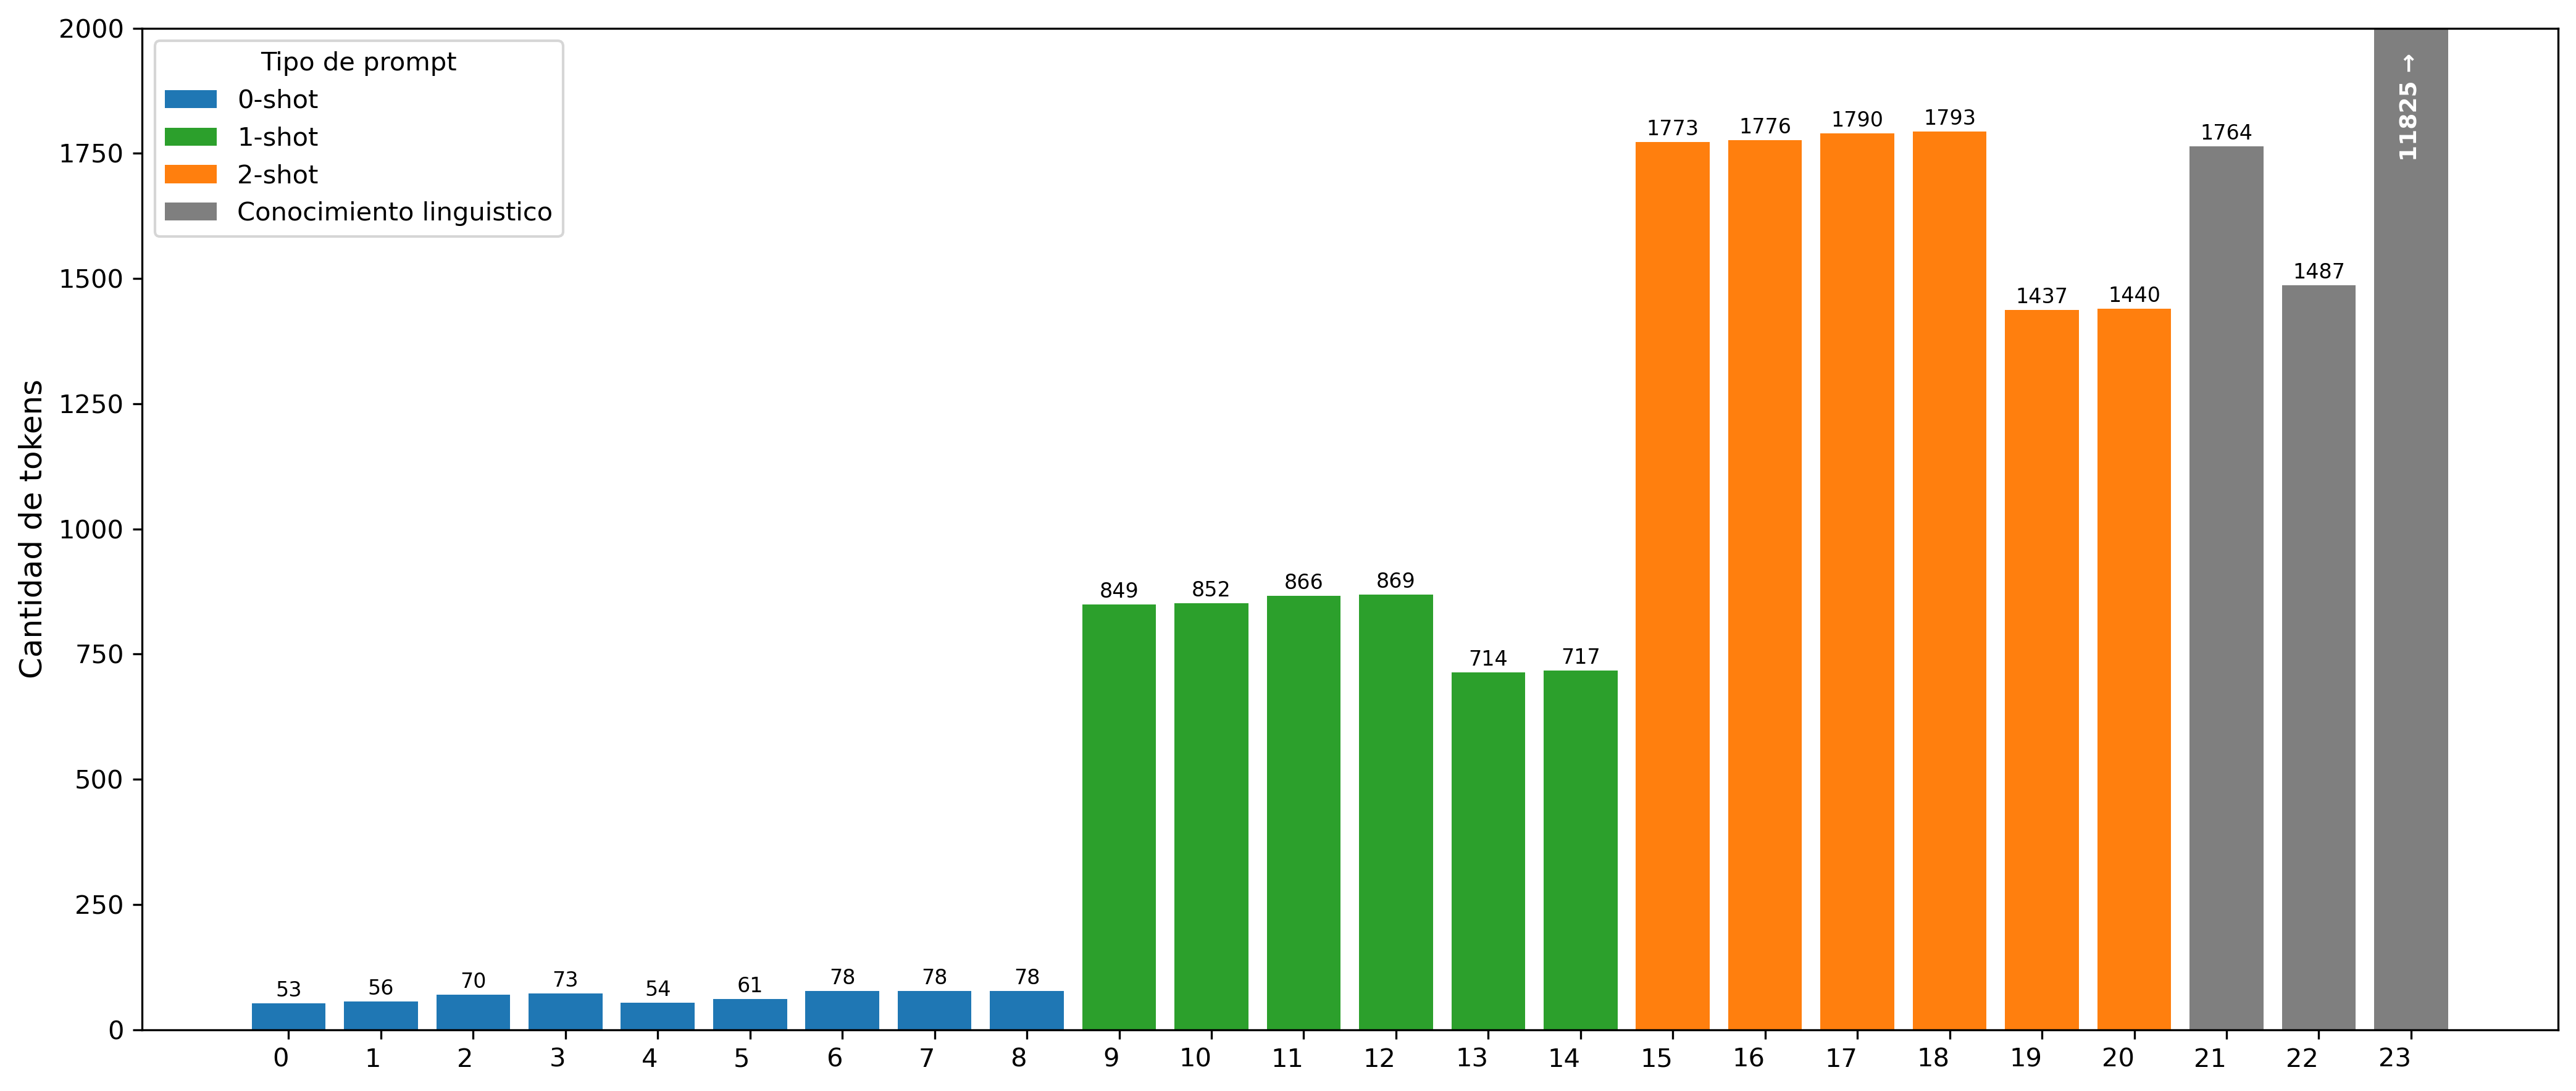
\includegraphics[width=\textwidth]{Graficos_Tesis/grafico_tokens.png}
  \caption{Cantidad de tokens de cada prompt utilizado en los experimentos de Clasificación.}
  \label{fig:grafico_tokens}
\end{figure}

\subsubsection*{Restricciones prácticas y diferencias entre modelos}

Debido a limitaciones presupuestarias y operativas, no fue posible aplicar la totalidad de las estrategias de prompting ni de evaluación de forma uniforme en todas las arquitecturas. En el caso de los modelos comerciales ChatGPT y DeepSeek, el acceso se gestionó a través de una colaboración externa, lo que restringió las pruebas exclusivamente a la modalidad 2-shot, dado que esta había exhibido el mejor desempeño preliminar entre las variantes sin fine-tuning. Asimismo, por razones de costo, estos dos modelos se evaluaron únicamente sobre las particiones de evaluación eval y holdout. Cabe destacar que los experimentos en ambas particiones se ejecutaron con una diferencia temporal considerable, lo que introdujo variaciones significativas en las métricas obtenidas debido a la evolución interna de las API.

Por otro lado, la herramienta especializada Cathoven solo pudo ser evaluada en los conjuntos de evaluación (eval), quedando fuera de las pruebas sobre la partición de holdout por restricciones de tiempo en las etapas finales del trabajo. Por este motivo, sus resultados no se exponen en la discusión principal de este documento, aunque los datos obtenidos para eval se encuentran disponibles en el \Cref{sec:tab_res}.

En cuanto a los modelos de código abierto, ciertas arquitecturas como Gemma 2 9B evidenciaron limitaciones en su ventana de contexto que impidieron procesar los prompts más extensos. El consecuente truncamiento de las entradas imposibilitó la finalización adecuada de algunas pruebas, un factor crítico que se traduce en ciertos comportamientos anómalos que se analizan detalladamente más adelante.

Finalmente, la plataforma de evaluación Text Inspector presenta una restricción técnica por la cual no procesa textos que contengan menos de 100 palabras. En consecuencia, todas las muestras del corpus que cumplían con esta condición fueron clasificadas automáticamente bajo una categoría genérica de ``sin categoria'' para este modelo.

\subsection{Métodos y Métricas de Evaluación}\label{subsection:clas_metrica}
La evaluación del desempeño de los modelos de lenguaje en la tarea de clasificación automática según los niveles del CEFR requiere un conjunto de métricas que capture tanto la precisión general como aspectos más finos del comportamiento del modelo. Dado que los niveles CEFR presentan una estructura ordinal en la que las distancias entre niveles tienen un significado educativo concreto, algunos errores son más graves que otros. Por ejemplo, confundir un texto de nivel A2 con uno de nivel C1 tiene un impacto pedagógico mayor que confundirlo con B1. Por este motivo, la estrategia de evaluación adoptada combina métricas estándar de clasificación multiclase con métricas diseñadas específicamente para este dominio.

\subsubsection*{Métricas estándar}
Para obtener una medida general del rendimiento de cada modelo se utilizó la métrica más adoptada en la literatura de clasificación:

\paragraph{Accuracy}
Mide la proporción total de predicciones correctas sobre el conjunto de ejemplos evaluados. Es sencilla de interpretar, pero trata todos los errores por igual y no considera el balance entre clases, lo cual resulta problemático en datasets donde ciertos niveles CEFR están sobrerrepresentados.

\subsubsection*{Accuracy adaptada al dominio CEFR}
Si bien las métricas tradicionales permiten comparar modelos en términos generales, no capturan el hecho de que ciertos errores son pedagógicamente menos problemáticos que otros. Para abordar esta limitación, desarrollamos una métrica adicional que incorpora la estructura ordinal del CEFR.

\paragraph{Accuracy Aproximada}
Diseñada específicamente para este trabajo, asigna 0.5 puntos a aquellas predicciones que se encuentran a un nivel de distancia de la clase real. Esta métrica refleja mejor el impacto real de los errores en contextos educativos: entregar a un estudiante B1 un texto B2 puede ser adecuado o incluso beneficioso, mientras que entregar uno C2 resulta inadecuado.

Como se verá más adelante en \Cref{subsection:ad_metricas} adaptación existe una correspondencia conceptual directa entre el RMSE y la Accuracy Aproximada propuesta en este trabajo: ambas asumen la estructura ordinal del CEFR. Sin embargo, lo hacen desde perspectivas complementarias. El RMSE opera en el espacio del error continuo, penalizando de manera cuadrática las predicciones severamente desviadas. Por el contrario, la Accuracy Aproximada introduce una noción de recompensa parcial en el espacio discreto, asignando valor pedagógico a los errores marginales.

\subsubsection*{Criterios de reporte de resultados}
Con el objetivo de garantizar la consistencia metodológica y permitir una comparación equitativa entre las diferentes arquitecturas, en el capítulo de resultados se exponen únicamente las métricas obtenidas sobre la partición de holdout. Debido a las restricciones operativas y de acceso detalladas en la sección anterior, la disponibilidad de datos varía según el modelo: mientras que algunas variantes disponen de registros para la totalidad del dataset, otras se limitan a combinaciones específicas de las particiones de entrenamiento, evaluación o holdout, o bien exclusivamente a esta última. A fin de preservar la claridad en el cuerpo principal del texto, el desglose completo de los rendimientos en las fases de train y eval para cada configuración evaluada se ha trasladado al \Cref{sec:tab_res}.

\subsection{Fine-tuning}\label{subsection:clas_finetuning}
A partir de los resultados obtenidos en los experimentos basados en prompting, observamos que los LLMs open-source presentan limitaciones para capturar con precisión las diferencias entre niveles CEFR, especialmente en los casos donde los niveles son adyacentes (por ejemplo, B1 vs. B2) o cuando el contenido del texto presenta estructuras con alta variabilidad temática o estilística. Estos hallazgos motivaron la segunda fase del estudio: la adaptación específica de un modelo de lenguaje mediante fine-tuning, con el objetivo de mejorar su sensibilidad a las características lingüísticas relevantes para la clasificación CEFR.

\subsubsection*{Preparación del conjunto de datos}
Para entrenar un clasificador robusto, construimos un conjunto de datos adaptado al problema, compuesto por textos anotados con los seis niveles del CEFR (A1-C2). Como paso previo al entrenamiento, realizamos las siguientes acciones:

\begin{itemize}
    \item \textbf{Normalización de etiquetas:} cada nivel CEFR se mapeó a una etiqueta numérica entre 0 y 5.
    \item \textbf{Partición del dataset:} organizamos los datos en una estructura DatasetDict con particiones de train y eval.
    \item \textbf{Homogeneización de formato:} todos los textos fueron convertidos a un formato consistente, eliminando metadatos o artefactos irrelevantes presentes en los corpus originales.
\end{itemize}

Dado que la clasificación CEFR es sensible a pequeñas variaciones lingüísticas, fue fundamental preservar las características sintácticas y léxicas originales de los textos. No se aplicaron técnicas de data augmentation, para evitar introducir ruidos estructurales que afectan la calidad del entrenamiento.

\subsubsection*{Esquema de prompting instructivo para entrenamiento}
A diferencia de los enfoques sin fine-tuning, donde el prompt es procesado en tiempo de inferencia, en esta etapa optamos por un prompt instructivo fijo, incorporado directamente en el proceso de preprocesamiento. Este prompt se utilizó para garantizar que el modelo recibiera una instrucción clara y uniforme en cada ejemplo. La plantilla general fue:

\begin{quote}
``you are an English teacher and I want you to classify the following text for reading comprehension according to the CEFR classes, keep in mind that the label 0 is A1, label 1 is A2, label 2 is B1, label 3 is B2, label 4 is C1, label 5 is C2:
\{texto\}''  
\end{quote}

Esta estrategia contribuyó a que el modelo convergiera más rápidamente y a que interpretara de manera unívoca las etiquetas numéricas durante el entrenamiento y evaluación.

\subsubsection*{Arquitectura y parámetros de entrenamiento}
Como modelo base seleccionamos Meta-Llama-3.1-8B-Instruct, debido a su buen rendimiento en experimentos previos, su solidez en tareas relacionadas con análisis lingüístico y su equilibrio entre tamaño y capacidad expresiva. Para ajustarlo a la tarea CEFR:
\begin{itemize}
    \item Se agregó luego de la capa de salida del modelo una capa lineal con 6 neuronas, correspondiente a las seis clases CEFR.
    \item Se aplicó fine-tuning parcial, congelando todos los parámetros del modelo excepto la capa clasificadora. Esta estrategia permitió:
    \begin{itemize}
        \item reducir significativamente los costos computacionales,
        \item mitigar el riesgo de overfitting,
        \item preservar el conocimiento lingüístico general del modelo.
    \end{itemize}
\end{itemize}

Los hiperparámetros utilizados fueron:
\begin{itemize}
    \item Optimizador: AdamW
    \item Learning rate: $1 \times 10^{-3}$
    \item Batch size efectivo: 8 $\times$ gradiente acumulado cada 4 pasos
    \item Épocas: 30
    \item Loss function: entropía cruzada
    \item Regularización: sin dropout adicional, weight decay = 0,
    
    label smoothing = 0
    \item Métrica principal de selección: Accuracy
    \item Ventana de contexto: 15000 tokens
\end{itemize}

\subsubsection*{Adaptación de prompts y coherencia entre etiquetas}
Como variante adicional, exploramos una versión de los experimentos donde los prompts de entrada se enriquecieron con la instrucción explícita que vincula etiquetas numéricas con niveles CEFR.
\begin{quote}
``keep in mind that the label 0 is A1, label 1 is A2, label 2 is B1, label 3 is B2, label 4 is C1, label 5 is C2''
\end{quote}

Esta modificación buscaba eliminar confusiones del modelo sobre la codificación interna de categorías. La adaptación resultó beneficiosa tanto en entrenamiento como en evaluación, contribuyendo a predicciones más estables entre niveles adyacentes.

\subsection{Análisis de Resultados}\label{subsection:clas_resuslt}
En esta sección presentamos y analizamos los resultados obtenidos en los experimentos de clasificación automática de textos según los niveles del CEFR. El objetivo es comparar el rendimiento de los distintos enfoques evaluados, prompting, prompting con conocimiento lingüístico, modelos libres, privativos y fine-tuning, así como entender en qué condiciones cada estrategia resulta más eficaz. A lo largo del análisis mostramos cómo las aproximaciones basadas en fine-tuning superan sistemáticamente al resto de alternativas, y discutimos los factores que explican estas diferencias.

\paragraph{Comparación general entre modelos con y sin fine-tuning}

En la Figura \ref{fig:finetuning} se observa una diferencia clara y consistente entre el modelo ajustado mediante fine-tuning y aquellos evaluados únicamente con estrategias de prompting (incluyendo prompting pedagógico, descriptores CEFR y prompting con conocimiento lingüístico).

El modelo con fine-tuning alcanza niveles de precisión considerablemente superior, lo que evidencia la importancia de adaptar los LLMs preentrenados al dominio específico de clasificación CEFR.

\begin{figure}[H]
  \centering
  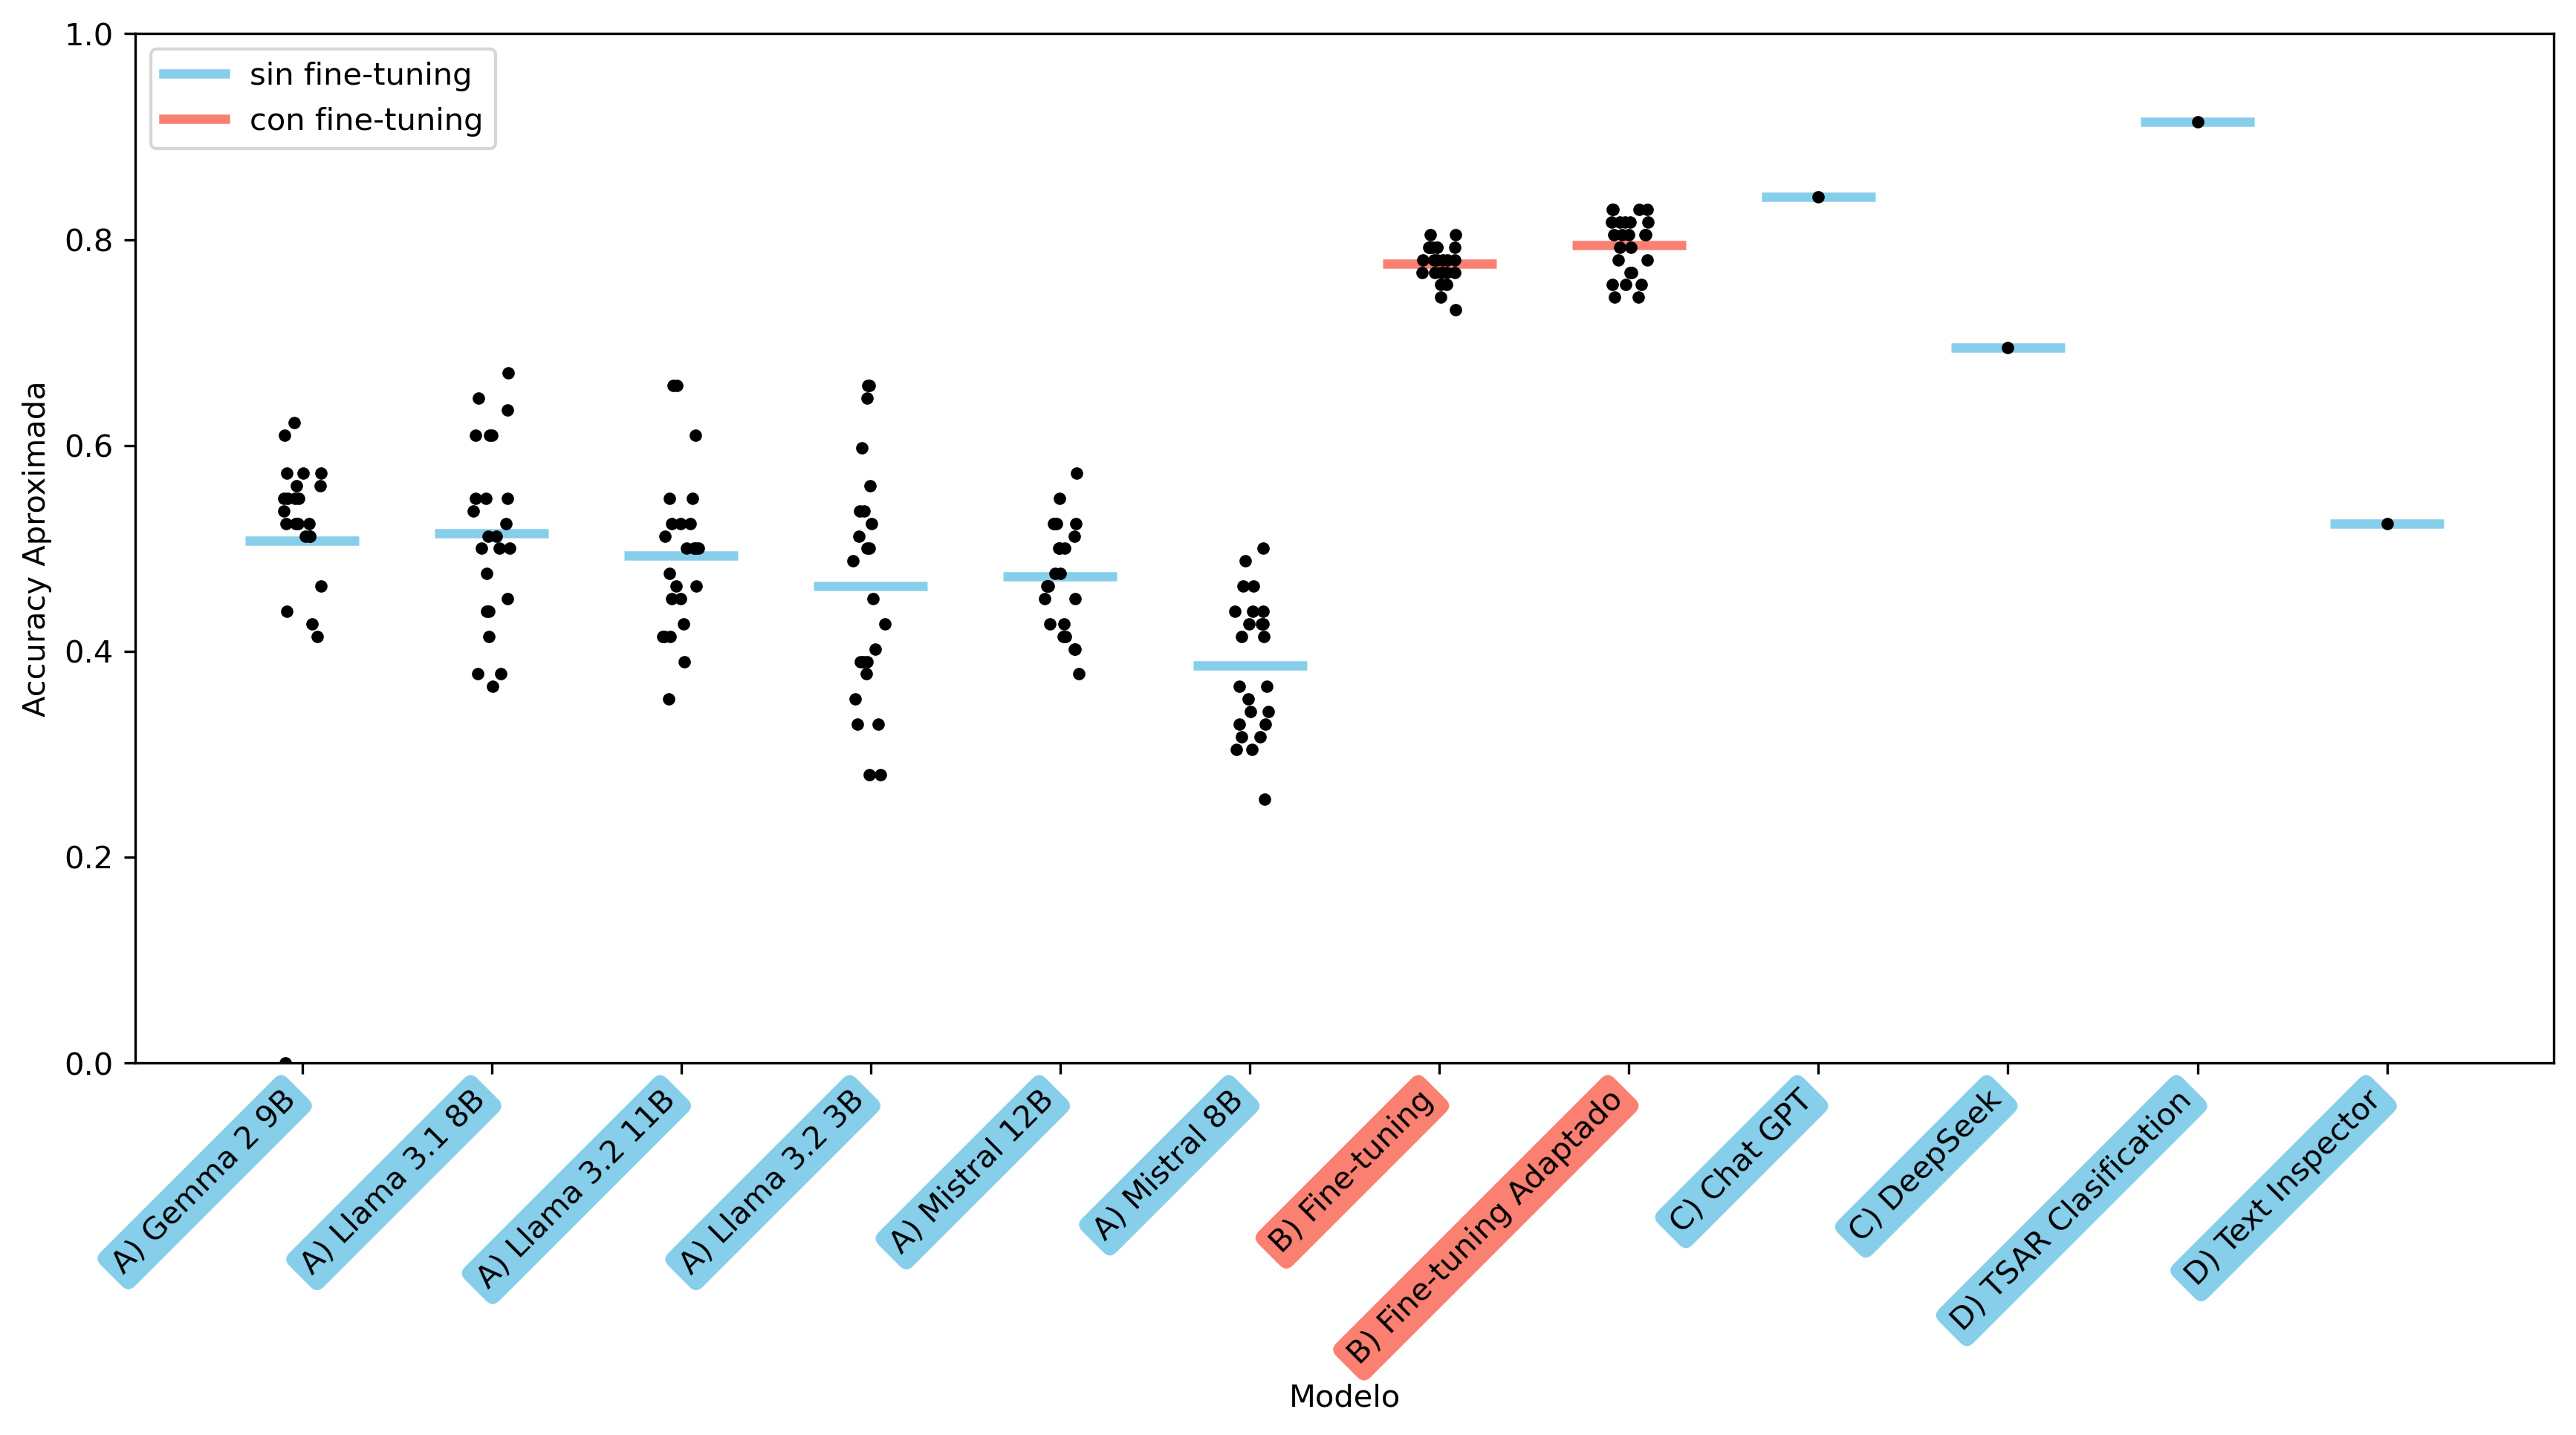
\includegraphics[width=\textwidth]{Graficos_Tesis/custom_dataset_holdout_con_finetuning_vs_sin_Accuracy_aprox.png}
  \caption{Acuraccy Aproximada de los modelos sin finetuning (celeste) vs modelos con finetuning propios (rojo), con promedio de todos los prompts usados}
  \label{fig:finetuning}
\end{figure}

\paragraph{Modelos privativos frente a modelos de código abierto}
La Figura~\ref{fig:privativos} presenta una comparación directa entre las arquitecturas abiertas y los modelos comerciales ChatGPT y DeepSeek. Debido a las restricciones operativas y de costos detalladas previamente, estos últimos solo fueron evaluados mediante el prompt 15, correspondiente a la estrategia de prompting con dos ejemplos seleccionados por docentes. 

Al analizar la partición de holdout, se observa un desempeño sobresaliente por parte de ChatGPT, que establece una diferencia amplia respecto a las demás alternativas. Es destacable que, en comparación con las pruebas iniciales, ChatGPT exhibe una mejora significativa en su accuracy aproximada dentro de este conjunto, mientras que DeepSeek mantiene un rendimiento estable y similar al registrado anteriormente. Por su parte, el clasificador de TSAR, incorporado como línea de referencia en la ilustración, continúa siendo el modelo con mejores métricas globales en toda la comparativa, un aspecto cuyo análisis detallado se posterga para las secciones subsiguientes.

\begin{figure}[H]
  \centering
  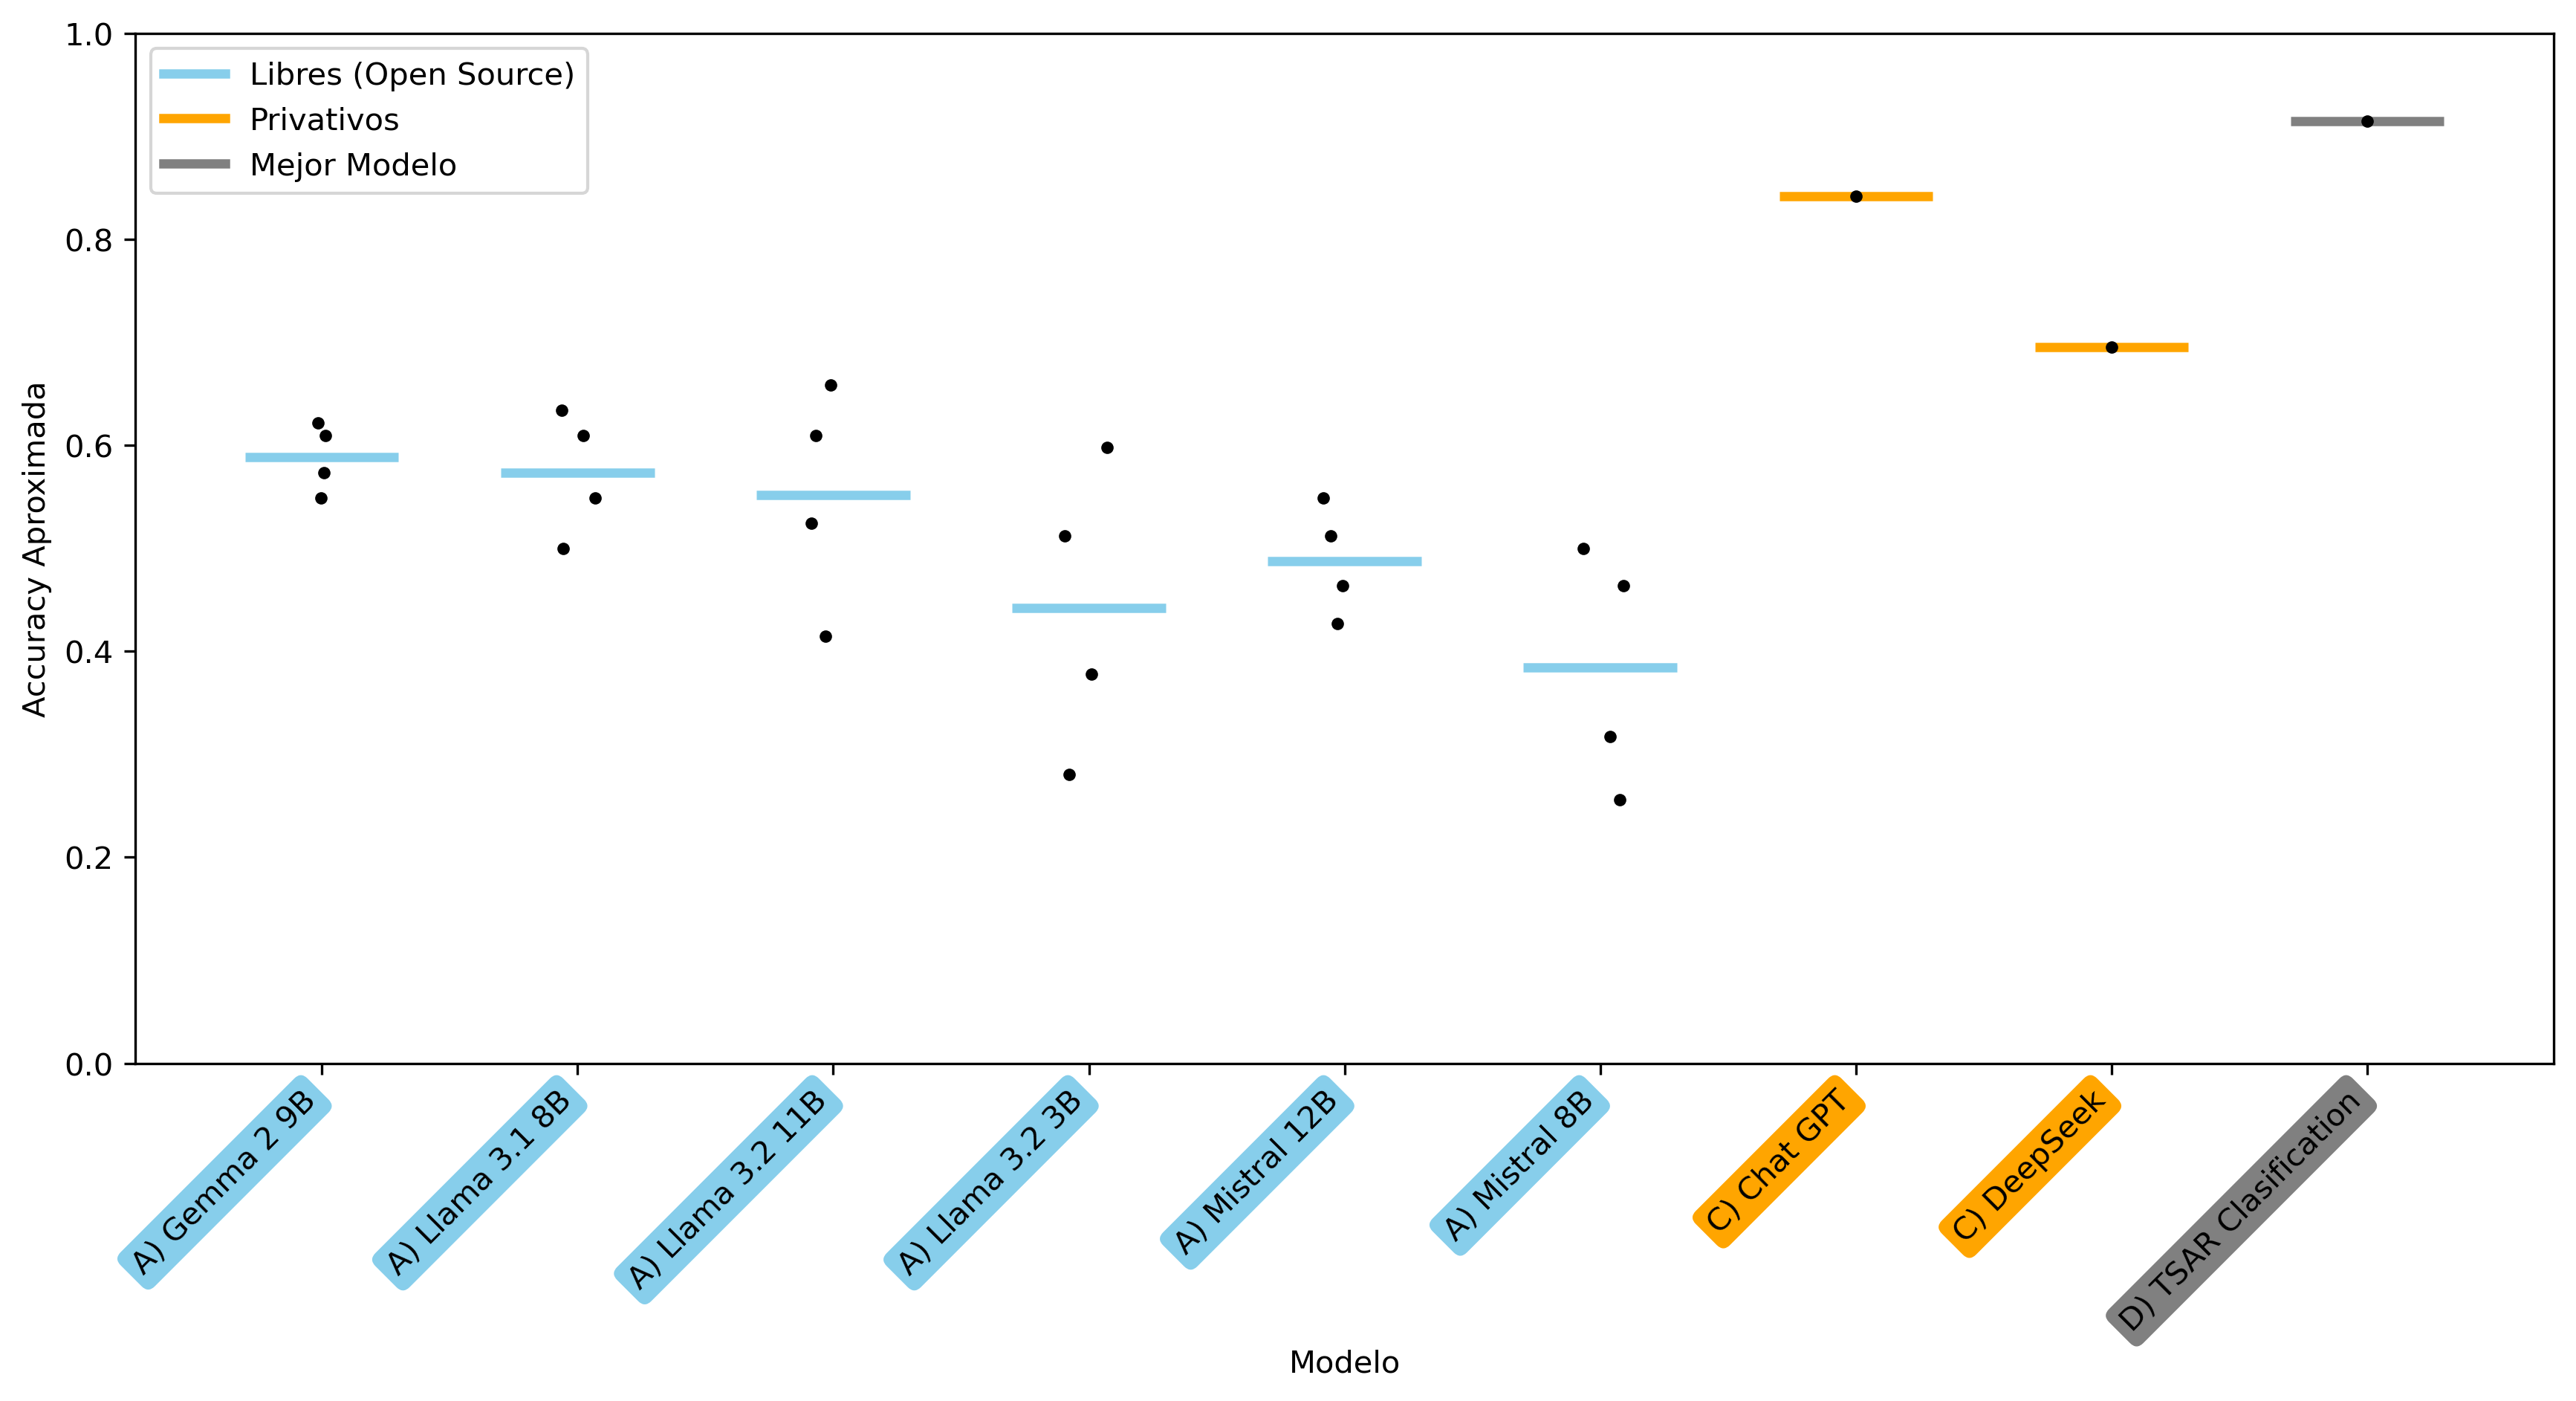
\includegraphics[width=\textwidth]{Graficos_Tesis/custom_dataset_holdout_privativo_vs_libre_acuraccy_aprox.png}
  \caption{Acuraccy Aproximada de los modelos libres (celeste) vs modelos privativos (naranja), con promedio de los prompts 15 a 18}
  \label{fig:privativos}
\end{figure}

Este comportamiento en holdout contrasta parcialmente con los resultados obtenidos en la partición de evaluación, cuyos datos no se visualizan en el gráfico, sino que se detallan en la tabla del \Cref{sec:tab_res}. En dicha partición de evaluación, los modelos privativos mostraban un rendimiento más homogéneo y apenas ligeramente superior a las variantes open-source sin fine-tuning. Esta ventaja inicial no resultaba determinante, dado que arquitecturas abiertas como LLaMA 3.1 8B y LLaMA 3.2 11B alcanzaban niveles de precisión comparables, consolidando la competitividad de las opciones de código abierto en instancias previas del experimento.

\paragraph{Comparación entre modelos open-source}

En la Figura \ref{fig:libres} se comparan los modelos libres. Una de las principales observaciones es que los valores promedio de accuracy se ubican dentro del rango 0.45-0.55. Luego LLaMA 3.1 8B y Gemma 2 9B obtienen las mejores medias de precisión. Ademas Mistral 12B presenta menor dispersión en los resultados, reflejando un comportamiento más estable, mientras que LLaMA 3.1 8B alcanza algunos de los valores máximos más altos de toda la comparación.

En función de estos resultados y considerando además su menor tamaño y requerimientos computacionales, se seleccionó el modelo LLaMA 3.1 8B como candidato principal para aplicar fine-tuning.

\begin{figure}[H]
  \centering
  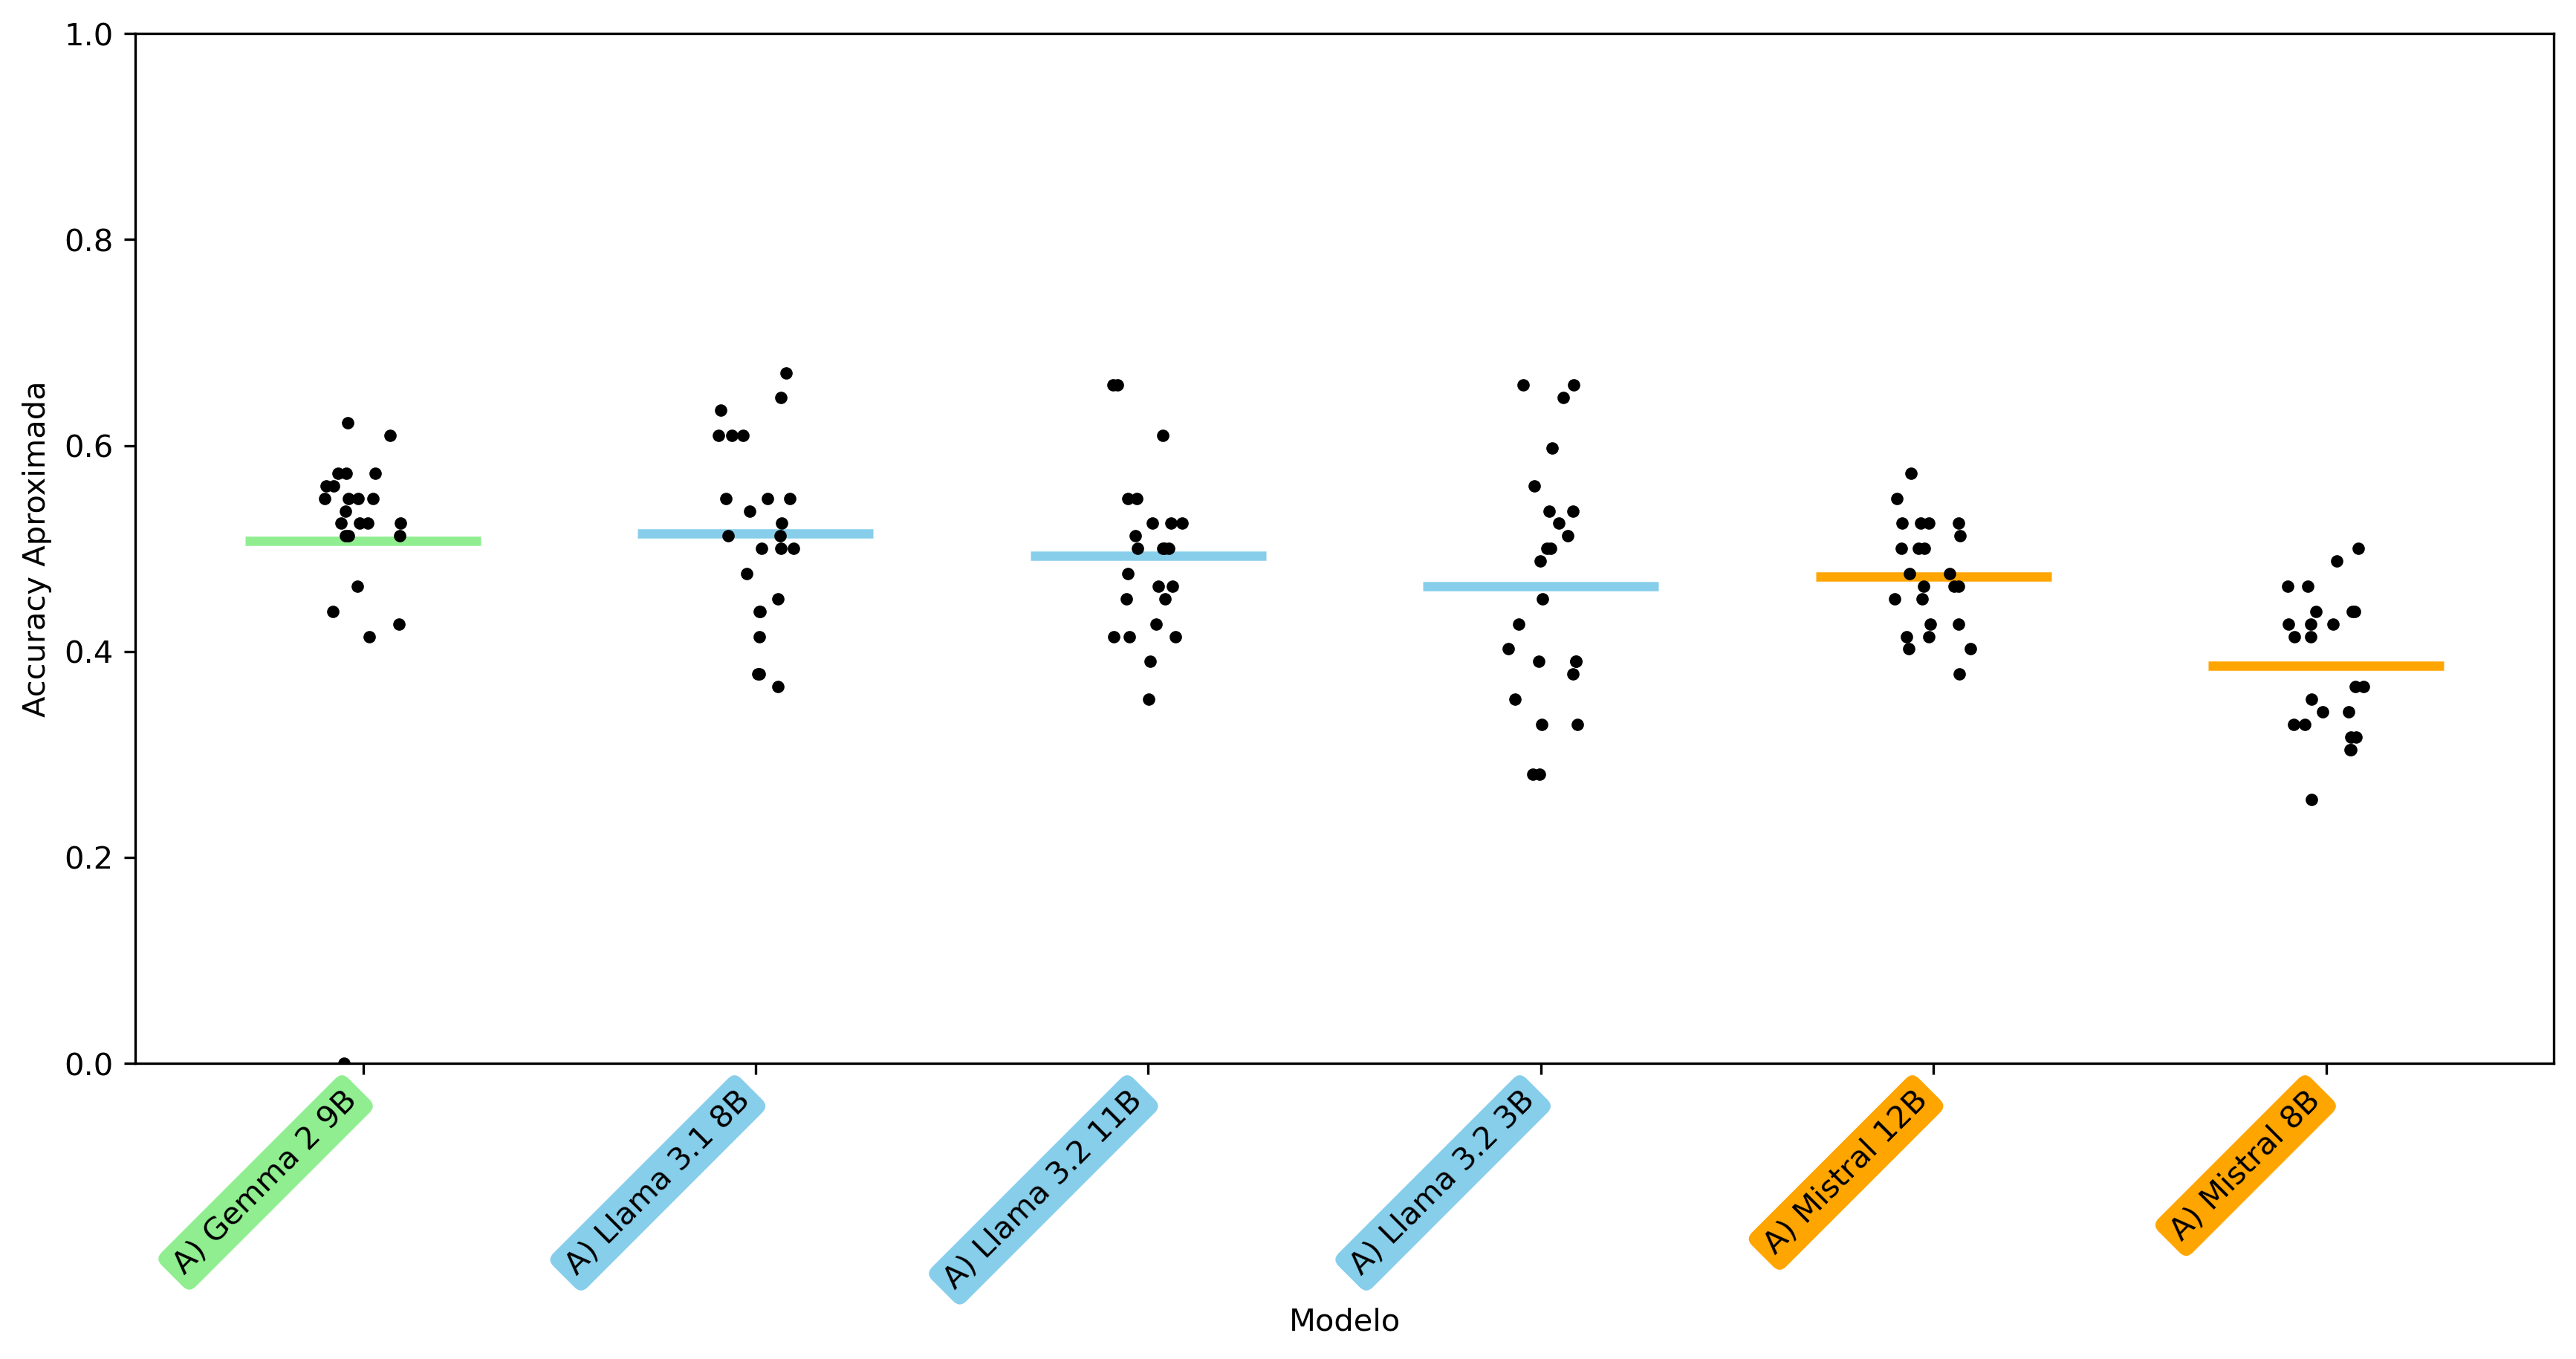
\includegraphics[width=\textwidth]{Graficos_Tesis/custom_dataset_holdout_differencias_entre_libres_acuracy_aprox.png}
  \caption{Acuraccy Aproximada de los modelos libres, con promedio de todos los prompts}
  \label{fig:libres}
\end{figure}

Por último hay que mencionar que estos resultados se mantienen para el resto de las particiones, el mejor promedio lo tiene el modelo LLaMA 3.1 8B y con muy poca diferencia estan Gemma 2 9B y Mistral 12B con valores similares.


\paragraph{Influencia del tipo de prompt y longitud del prompt}

La Figura \ref{fig:todos_los_modelos} y \ref{fig:modelos_ind} muestra el desempeño de los modelos comparando distintas estrategias experimentales (0-shot, 1-shot, 2-shot, prompting pedagógico, prompting con conocimiento lingüístico y variantes con corrección de sesgo).

Se puede obsevar que los modelos con fine-tuning mantienen ventaja incluso frente a prompts largos. Aunque la longitud del prompt introduce variabilidad, los modelos ajustados continúan obteniendo mejores resultados que cualquier configuración sin entrenamiento adicional.

La longitud excesiva del prompt puede degradar el rendimiento. Especialmente en prompting con conocimiento lingüístico, que requiere instrucciones más extensas y algunos modelos muestran una caída notable, posiblemente originada por efectos adversos en los mecanismos de atención (“olvido” parcial del contenido relevante). Este comportamiento se observa con mayor fuerza en modelos medianos como Mistral 3B o Gemma 2 9B.

Además para algunos prompt particulares se puede ver una caída en el rendimiento en comparacion a prompts similares, por ejemplo para los prompt 11, 12 (1-shot con correccion de sesgo) y prompt 17 y 18 (2-shot con correccion de sesgo) se puede observar una caída en el promedio del prompt en comparacion con prompts similares.

Las tendencias dependen del modelo.
\begin{itemize}
    \item Gemma 2 9B: en el experimento 23 obtiene accuracy 0 debido a una ventana de contexto insuficiente, luego tiene baja variabilidad sin mostrar un patron claro.
    \item LLaMA 3.1 8B: leve mejora progresiva de 0-shot $\rightarrow$ 1-shot $\rightarrow$ 2-shot.
    \item LLaMA 3.2 11B: comportamiento similar, aunque con menor gradiente de mejora.
    \item llama 3.2 3B: alta variabilidad, los prompts con correccion de sesgo parece influir negativamente.
    \item Mistral 12B: tiene variabilidad media, sin un patron claro.
    \item Mistral 8B: su rendimiento es el mas bajo, sin mostrar algun patron.
    \item Fine-tuning: muy poca variabilidad, resultados muy buenos.
    \item Fine-tuning adaptado: ligera mejora respecto a la versión sin adaptación, aunque con una variabilidad un poco mayor.
\end{itemize}

Estos resultados sugieren que, para algunos modelos, proporcionar más información no necesariamente mejora la predicción; en ciertos casos incluso introduce ruido estructural o saturación de contexto.

\begin{figure}[H]
  \centering
  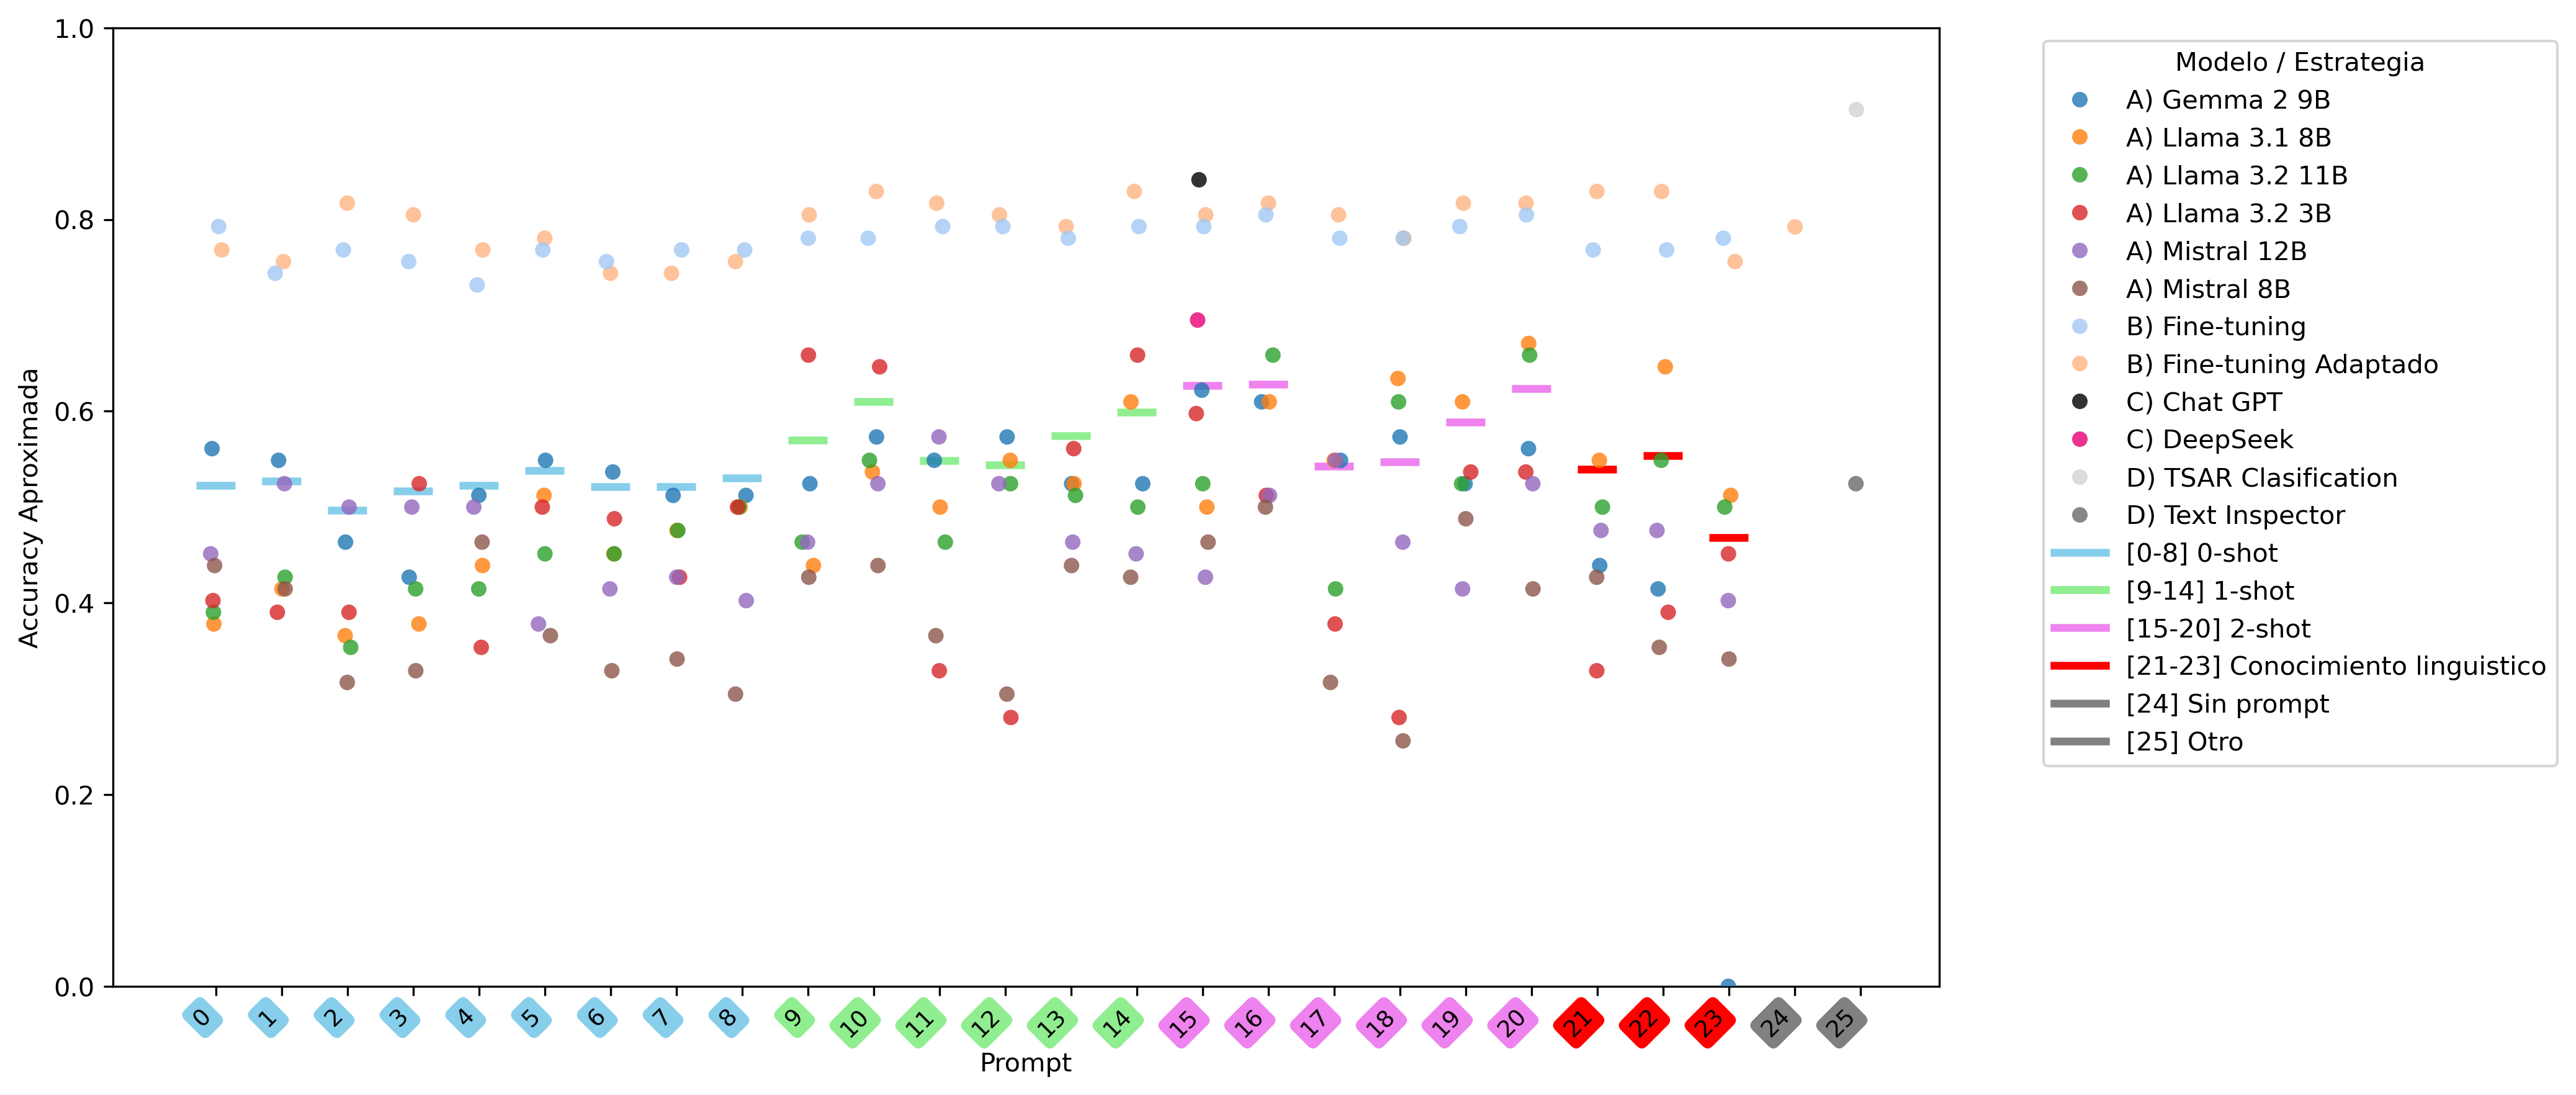
\includegraphics[width=\textwidth]{Graficos_Tesis/custom_dataset_holdout_experimentos_Accuracy_aprox.png}
  \caption{Acuraccy Aproximada de todos los experimentos realizados, con promedio de todos los modelos segun los prompts. Los resultados fueron coloreados segun el tipo de modelo, colores nitidos modelos libres, colores claros modelos con finetuning, colores oscuros modelos privativos y colores grises herramientas.}
  \label{fig:todos_los_modelos}
\end{figure}

\begin{figure}[H]
  \centering
  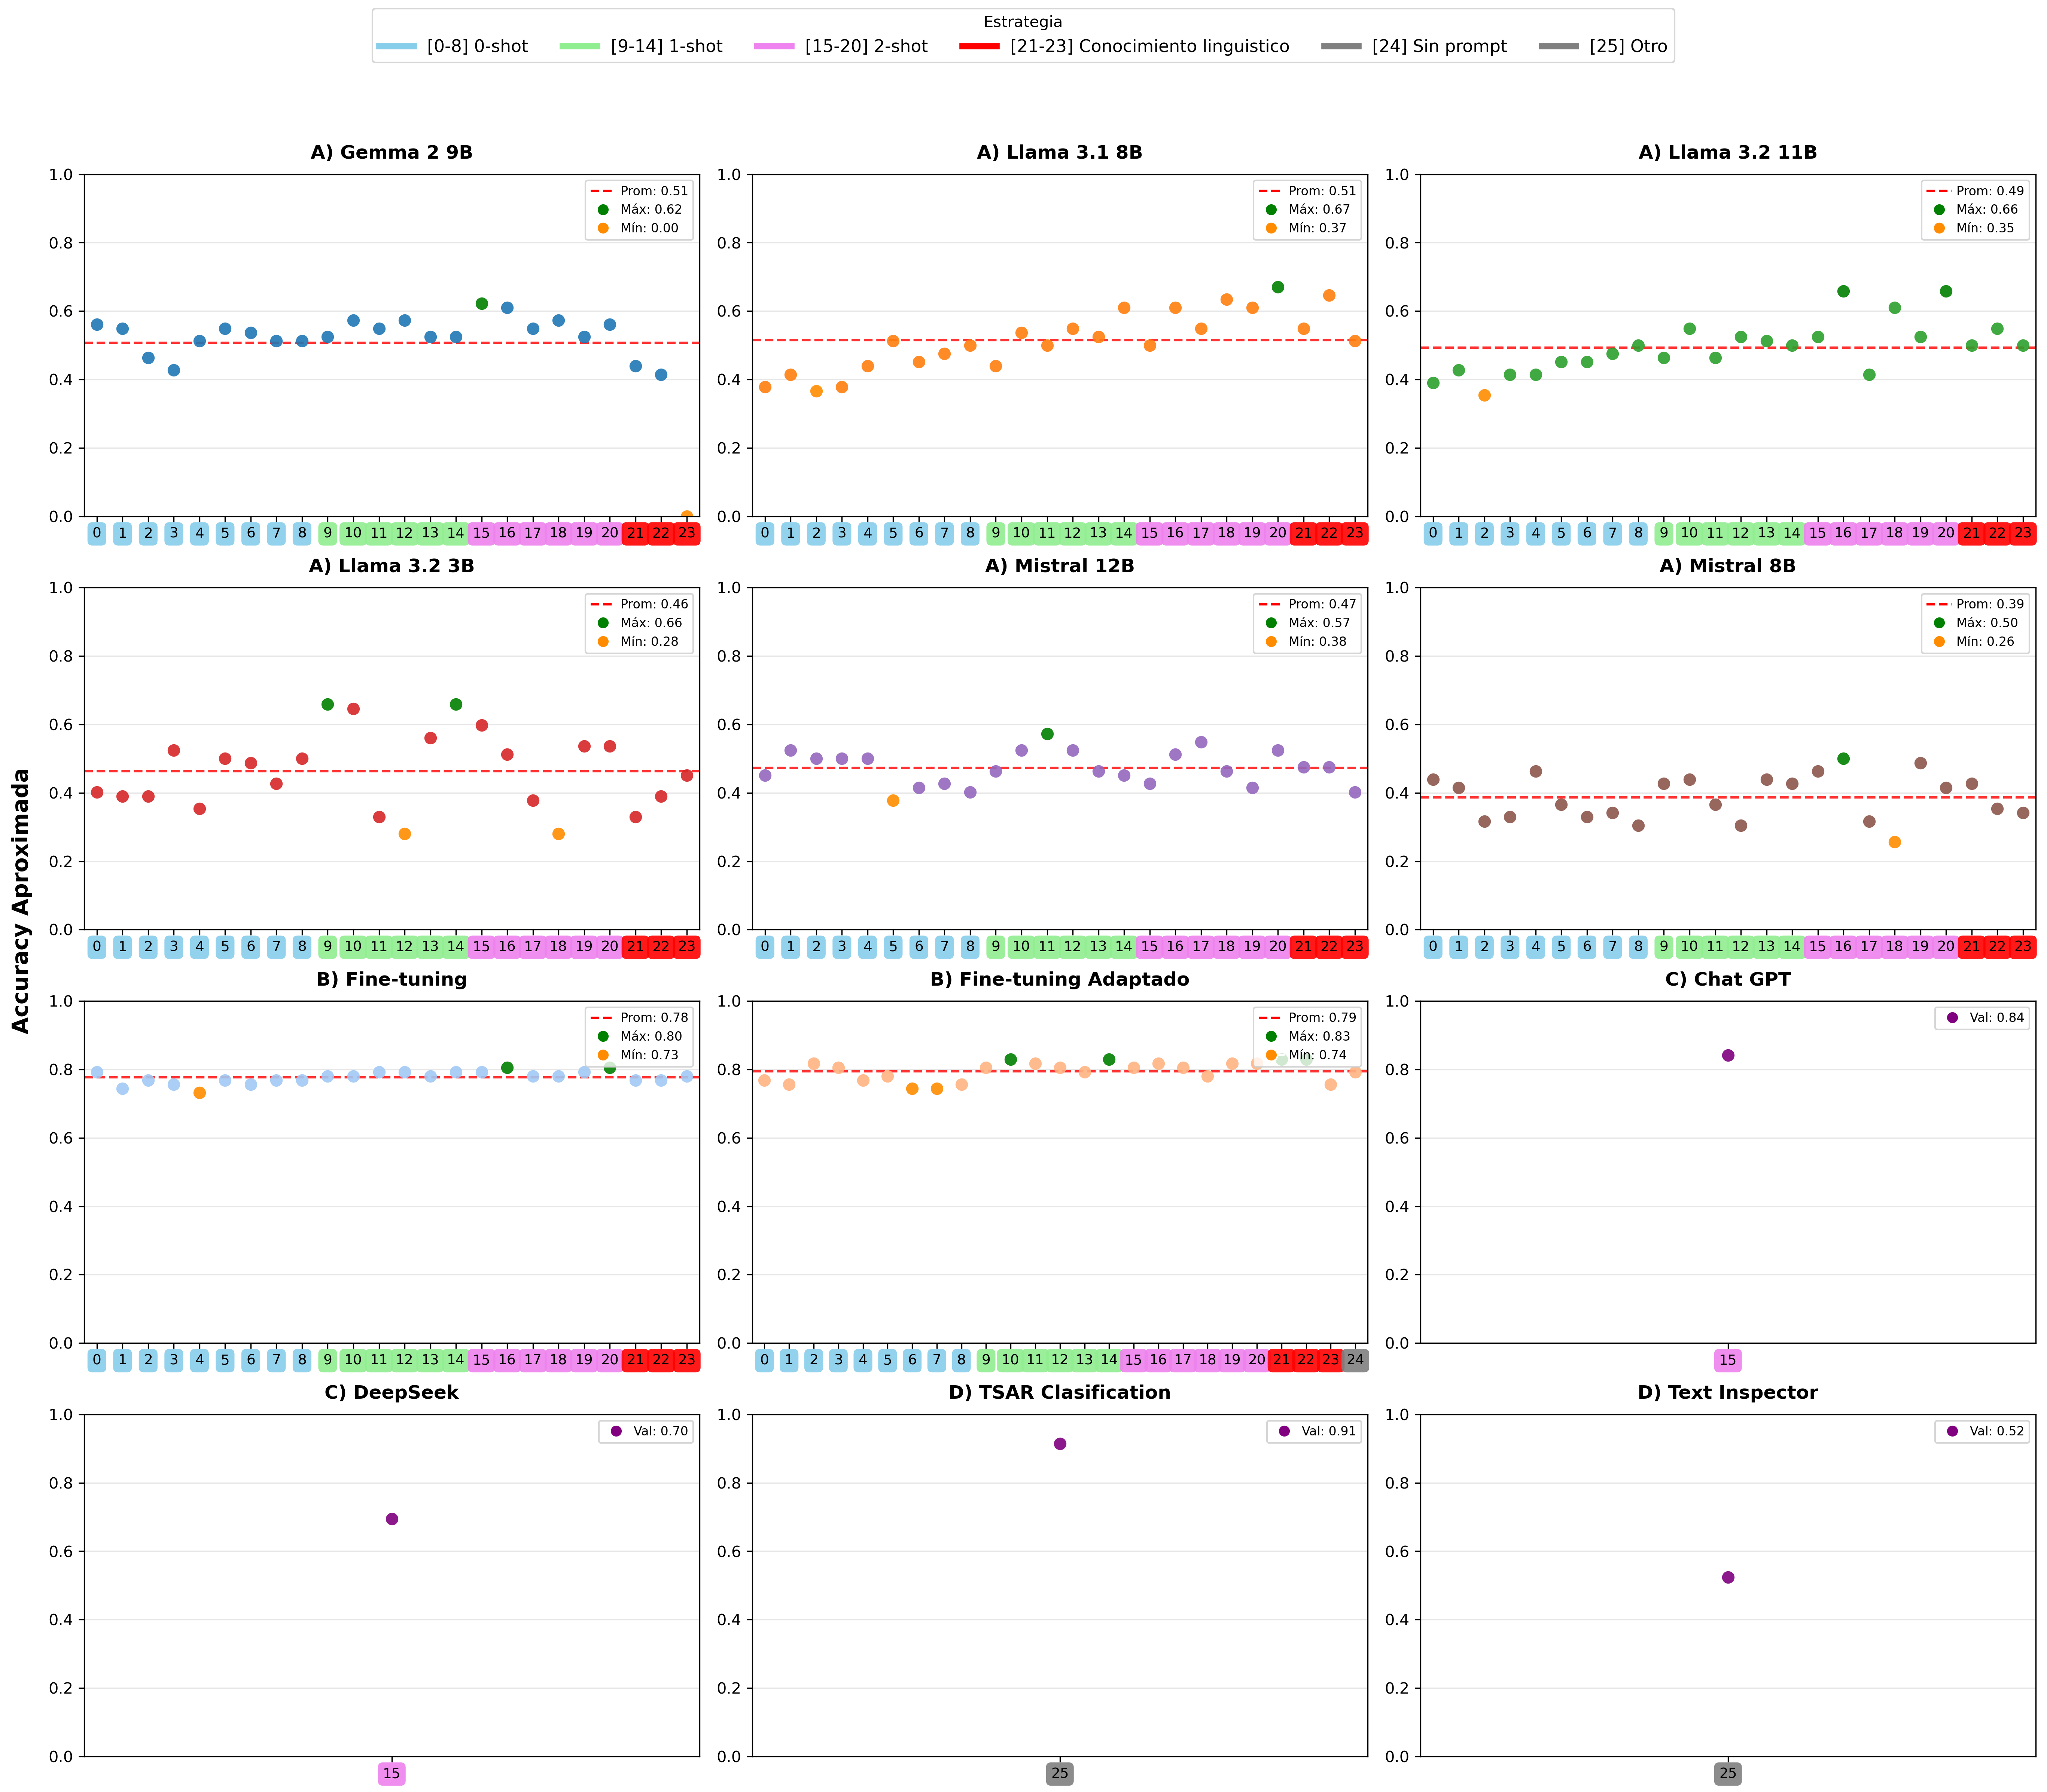
\includegraphics[width=\textwidth]{Graficos_Tesis/custom_dataset_holdout_stripplot_por_modelo.png}
  \caption{Acuraccy Aproximada de todos los experimentos realizados, separados por modelo.}
  \label{fig:modelos_ind}
\end{figure}

\revisar{
\paragraph{Análisis de Tablas de resultados}

En el \Cref{sec:tab_res} se muestran tablas detalladas con los resultados de cada modelo, cada prompt y cada particion del dataset. Estas tablas permiten un análisis más granular de las tendencias observadas en los gráficos anteriores, así como identificar casos específicos donde ciertos modelos o prompts presentan comportamientos atípicos.

MANTENGO ESTE PARRAFO?}

\paragraph{Preferencias de los modelos}

Anteriormente mencionamos que existian modelos que tenian una preferencia (bias) hacia categorias particulares, en el grafico \ref{fig:bias} podemos observar que todos los modelos tienen una clase que tiene sobre representacion con respecto de la distribucion original del dataset. Se puede ver que para Llama 3.1 8B, Llama 3.2 11B, Mistral 12B, tiene un bias sobre B2.

\begin{figure}[H]
  \centering
  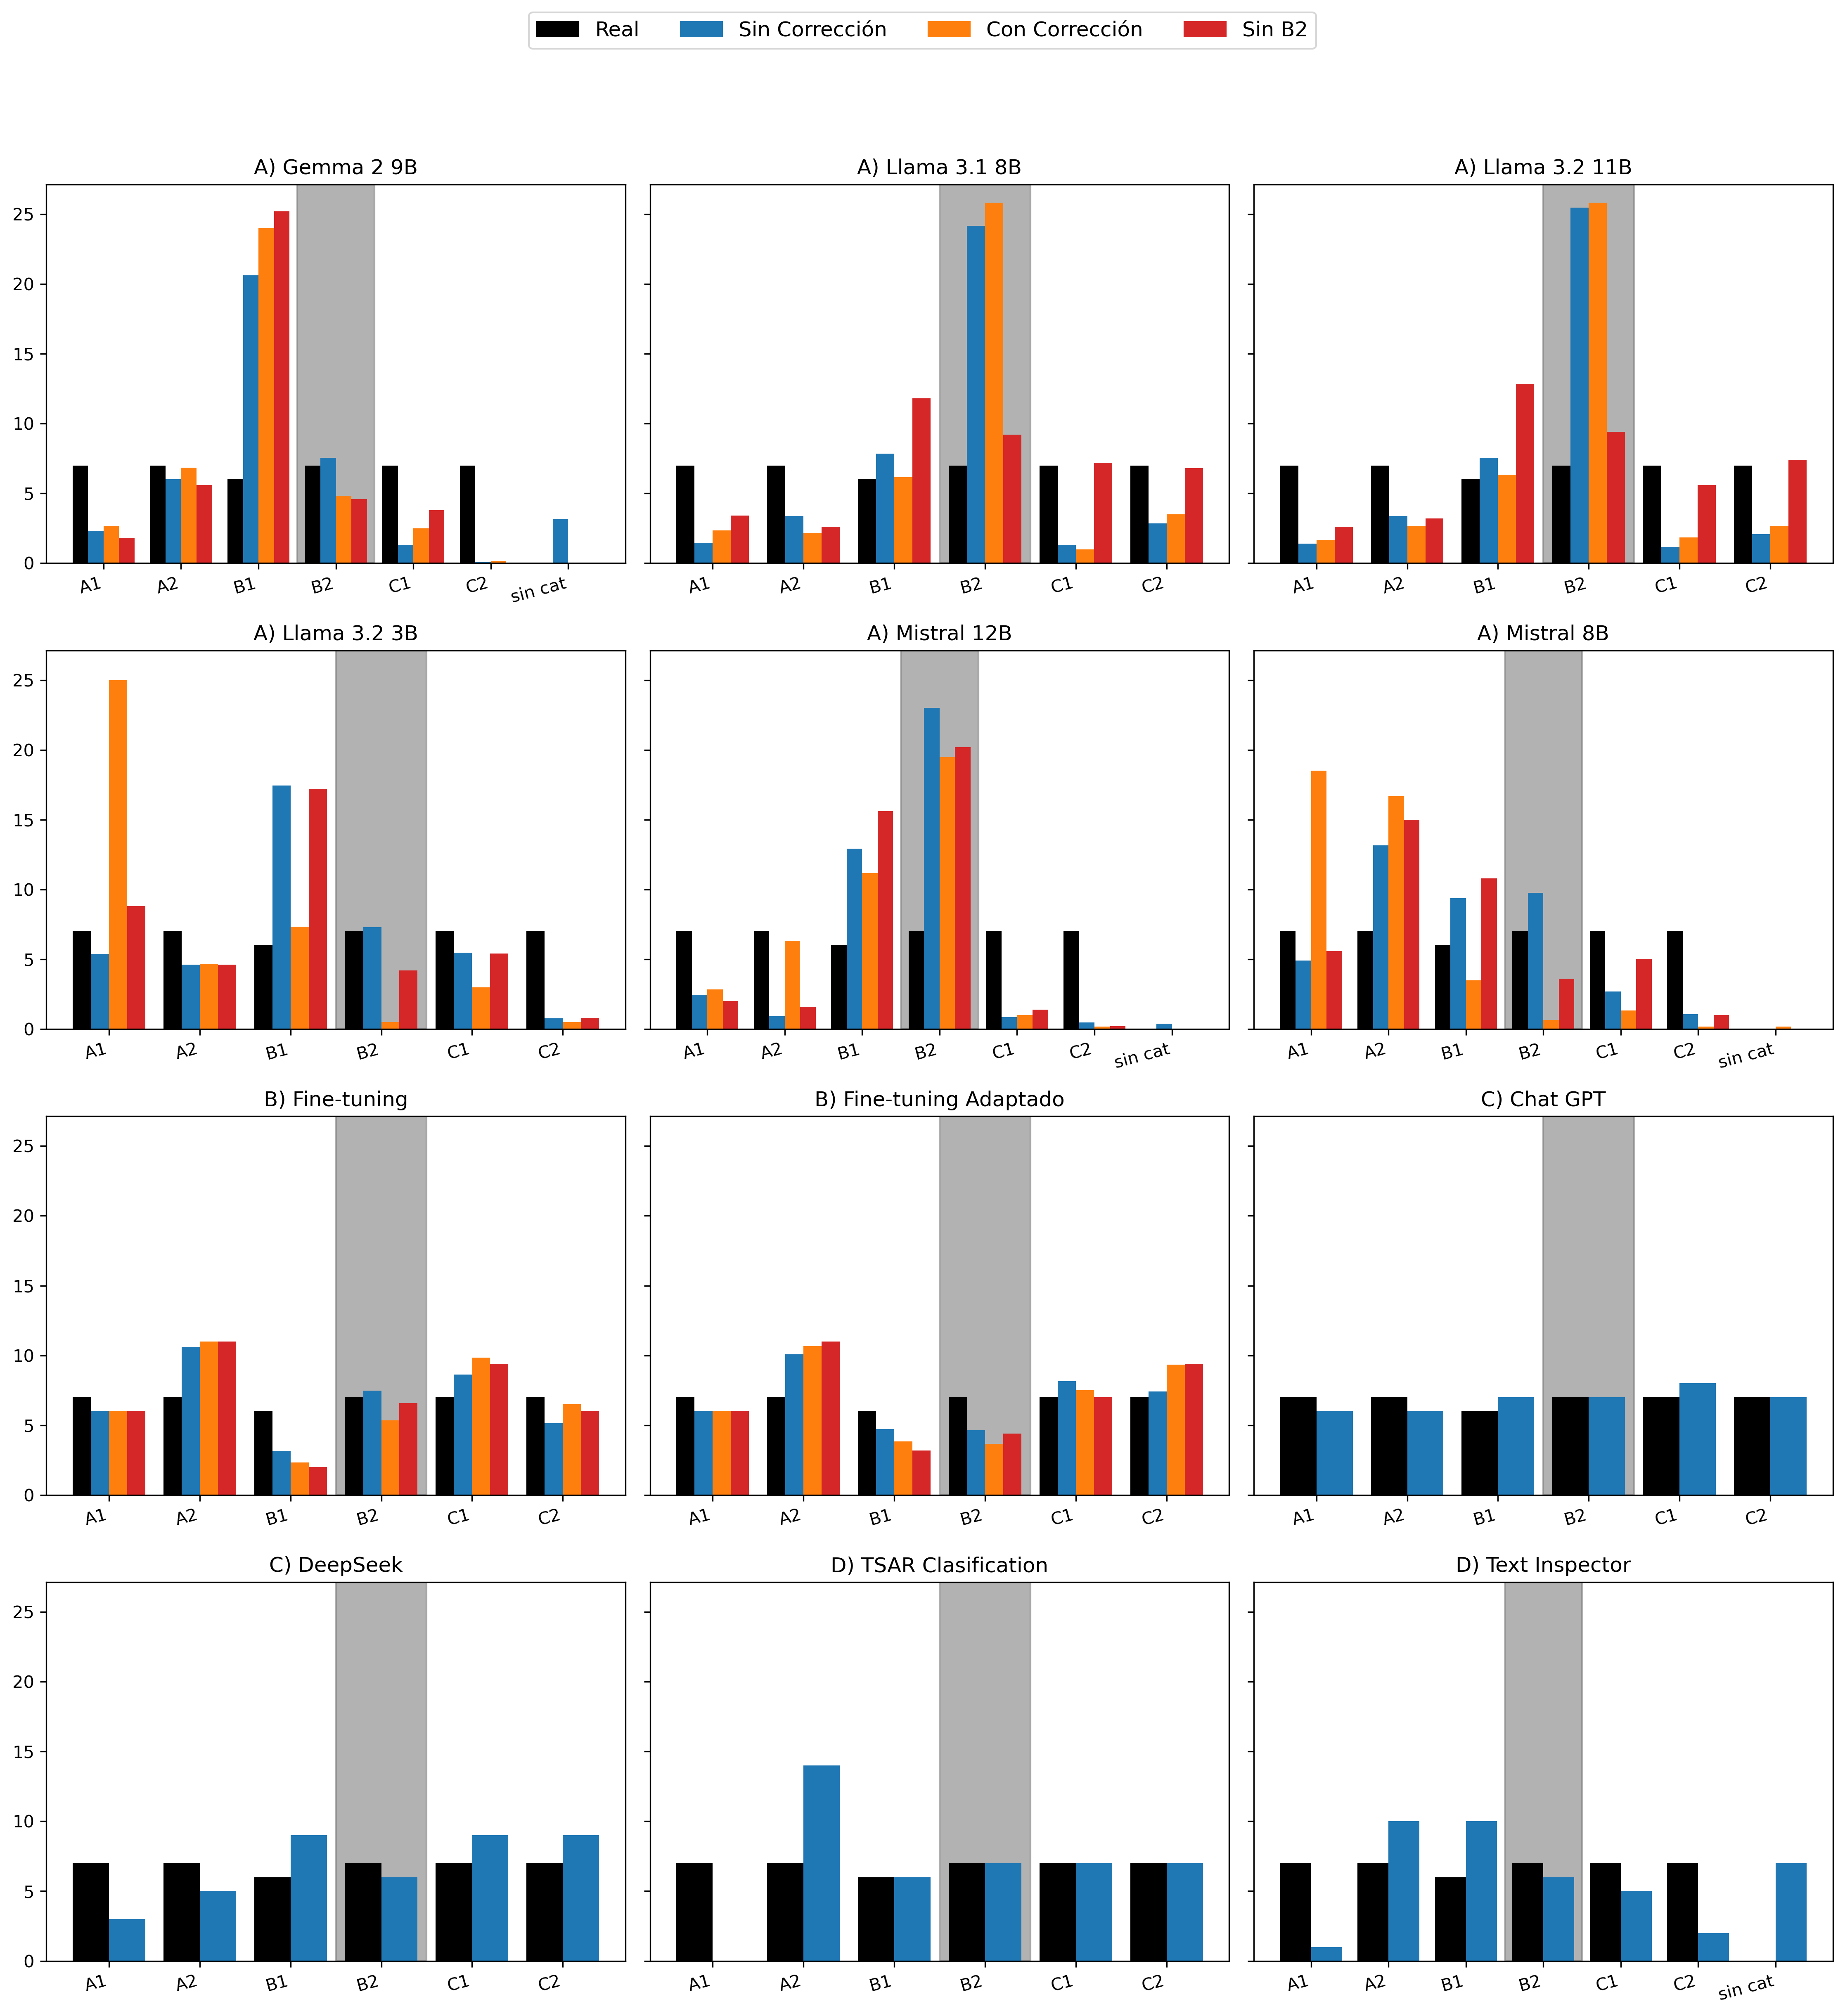
\includegraphics[width=\textwidth]{Graficos_Tesis/custom_dataset_holdout_bias.png}
  \caption{Cantidad de predicciones promedias hechas por cada modelo, agrupadas por el tipo de prompt. El area de B2 se ecuentra sobreada para una lectura mas facil. Sin cat significa que no se encontro una clasificacion valida}
  \label{fig:bias}
\end{figure}

Ademas se puede observar las categorias que tienen una baja representacion, como C2 para Gemma 2 9B o A1 para Llama 3.1 8B. Es de esperar que los extremos tengan una baja representacion, pero hay casos distintos como B2 para Llama 3.2 3B.

Para el caso de los modelos con finetuning tiene una distribucion mas similar a la original, pero se puede observar que hay una sobre representacion de A2 y baja representacion hacia B1, esto necesita un estudio particular sobre los textos de la particion de evaluacion que se estan clasificando mal de B1, ya que es posible que sean estructuralemente parecidos a los textos de A2 de la particion de entrenamiento, o sean distintos a los textos de B1 de la particion de entrenamiento. Tambien esta la posibilidad de que se encuentren mal clasificados, ya que no hay una clara distincion entre los niveles.


\paragraph{Matriz de confucion para los modelos}

En la tabla \ref{tab:mejores_prompts_modelos} se encuentra el mejor prompt segun su Aproximated Acuraccy de cada modelo. En esta tabla se puede observar que no hay un prompt que destaque en para todos los modelos, tampoco se puede encontrar una estrategia de prompting que sea ampliamente superadora a las demas, ya que esta tabla sugiere que varios modelos mejoran con 2-shot, pero no es definitiva para todos los modelo.

En el grafico \ref{fig:matriz_confucion} se encuentran las matrices de confucion para los experimentos anteriores, cada modelo con su mejor prompt. Se puede observar que cada modelo mantiene la tendencia que se ve en el grafico \ref{fig:bias}. Ademas se puede hacer foco en que es lo que no se desea en los modelos, lo primero es que su matriz de confucion sea disperza como la matriz de Mistral 8B y lo segundo es que hay algunos errores que son peores que otros, por ejemplo clasificar un texto como A2 siendo que su clasificacion original es C2 es un error mas severo que clasificar textos como B1 siendo originalmente A2, tanto por la proximidad como por la relacion de dificulad (una persona con nivel B1 deberia poder interpretar correctamente un texto de A2).

\begin{table}[H]
\centering
\resizebox{\linewidth}{!}{
\begin{tabular}{@{}cllcc@{}}
\toprule
Orden & Modelo & Prompt & Approximated Accuracy & Accuracy \\ \midrule
1 & D) TSAR Clasification & No toma Prompt & \textbf{0.915} & \textbf{0.829} \\
2 & C) Chat GPT & Prompt 15 & 0.841 & 0.707 \\
3 & B) Fine-tuning Adaptado & Prompt 22 & 0.829 & 0.707 \\
16 & B) Fine-tuning & Prompt 16 & 0.805 & 0.634 \\
52 & C) DeepSeek & Prompt 15 & 0.695 & 0.488 \\
53 & A) Llama 3.1 8B & Prompt 20 & 0.671 & 0.463 \\
54 & A) Llama 3.2 11B & Prompt 16 & 0.659 & 0.488 \\
55 & A) Llama 3.2 3B & Prompt 9 & 0.659 & 0.463 \\
61 & A) Gemma 2 9B & Prompt 15 & 0.622 & 0.390 \\
71 & A) Mistral 12B & Prompt 11 & 0.573 & 0.317 \\
89 & D) Text Inspector & No toma Prompt & 0.524 & 0.390 \\
112 & A) Mistral 8B & Prompt 16 & 0.500 & 0.341 \\
\bottomrule
\end{tabular}}
\caption{Mejor prompt para cada modelo según la Approximated Accuracy, para la partición de holdout.}
\label{tab:mejores_prompts_modelos}
\end{table}

\begin{figure}[H]
  \centering
  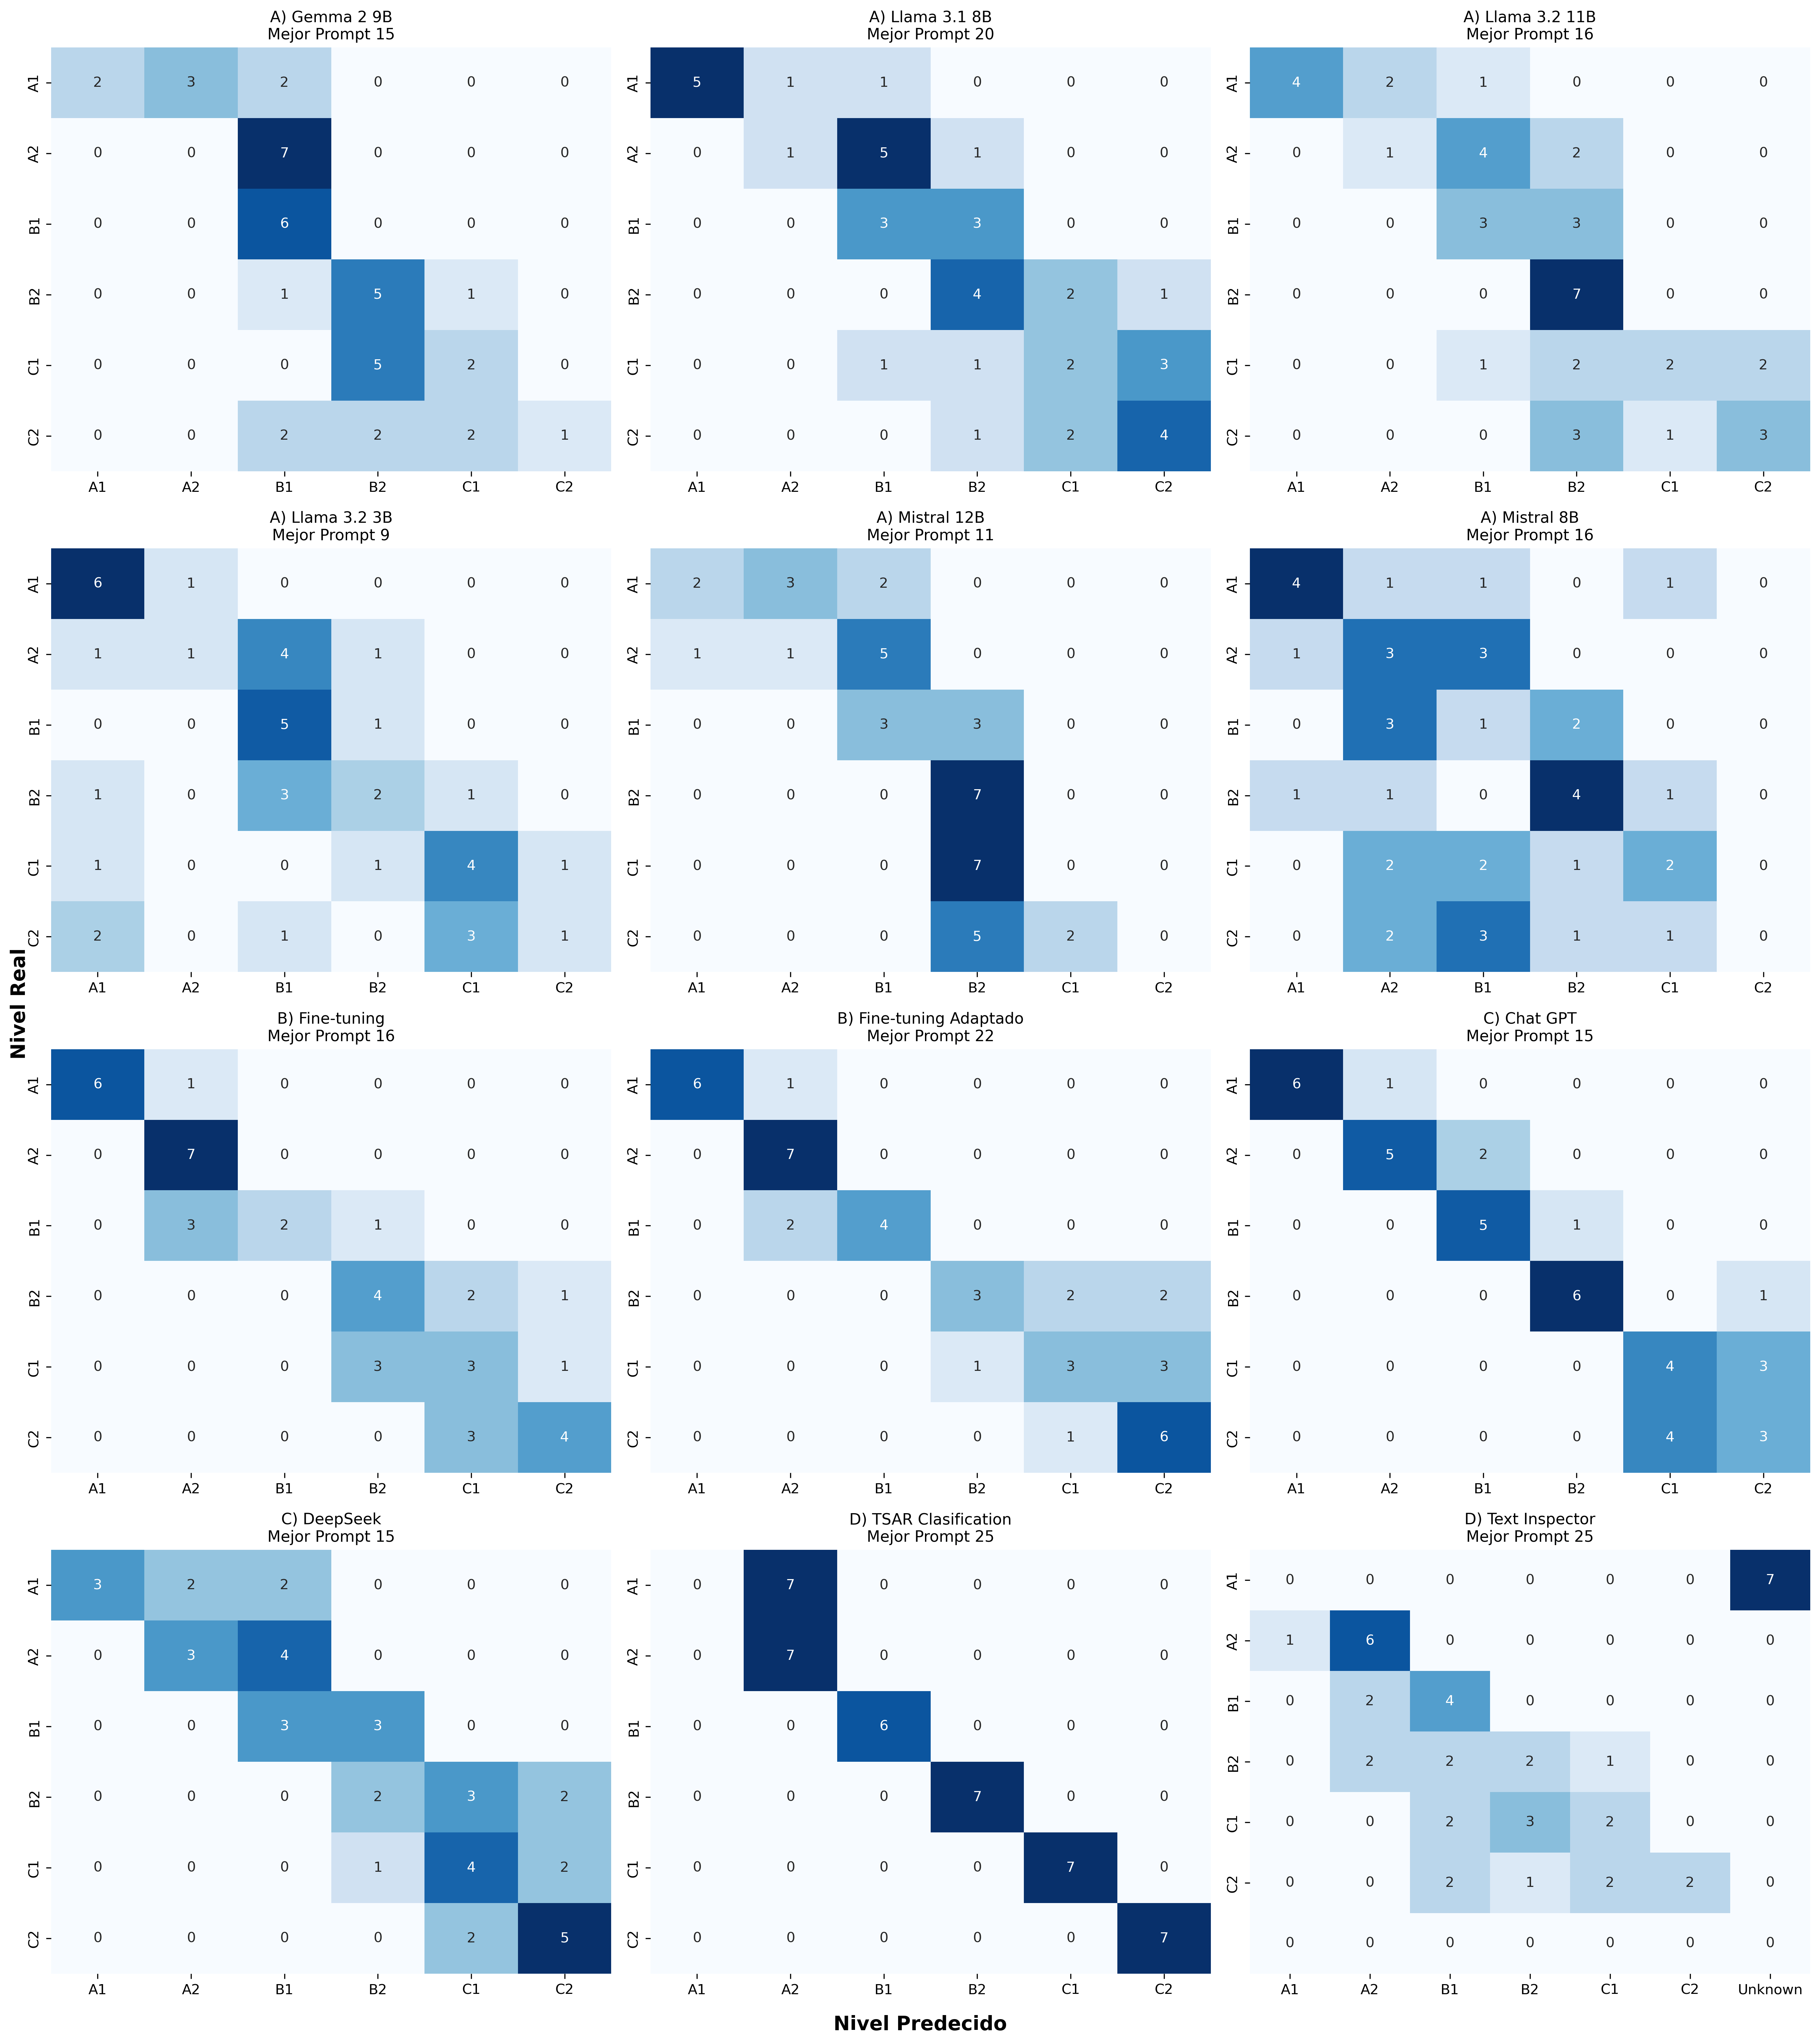
\includegraphics[width=\textwidth]{Graficos_Tesis/custom_dataset_holdout_todas_matrices.png}
  \caption{Matriz de confucion de todos los modelos, con su mejor prompt segun Aproximated Acuraccy.}
  \label{fig:matriz_confucion}
\end{figure}

\subsection{Discusión}\label{subsection:clas_discusion}

Los experimentos realizados demuestran que los modelos de lenguaje de gran tamaño generativos (de tipo decoder-only) son capaces de identificar de manera confiable el nivel del Marco Común Europeo de Referencia de un texto, particularmente cuando han sido sometidos a un fine-tuning. Los modelos ajustados superan sistemáticamente a todas las estrategias basadas en ingeniería de prompts.

Si bien el la ingeniería de prompts y el conocimiento linguistico, mejora ligeramente el desempeño en ciertos casos, también provoca una degradación en otros, lo que evidencia una notable variabilidad intermodelo. De hecho, la inconsistencia en los resultados de algunos modelos específicos llega a comprometer su confiabilidad para esta tarea.

Asimismo, la comparación entre prompts revela que, más allá de la variabilidad individual, existe una marcada tendencia en la mayoría de los modelos evaluados a sobreclasificar los textos en niveles intermedios (predominantemente en el nivel B2) y a infraclasificar las clases situadas en los extremos de la escala. Una de las causas subyacentes a este fenómeno podría ser el desbalance en el corpus de preentrenamiento; al igual que ocurre con el nivel A1, la escasez de material académico o literario representativo en los extremos de la distribución dificulta que el modelo generalice adecuadamente estas categorías.

Por otra parte, las mejoras en el rendimiento obtenidas mediante la optimización de prompts nunca alcanzan los niveles logrados a través del fine-tuning, incluso cuando este último se realiza con conjuntos relativamente pequeños de datos etiquetados. Este hallazgo subraya la importancia de la adaptación específica a la tarea, demostrando que el conocimiento lingüístico generalista de los modelos base es insuficiente si no se acompaña de una transferencia de aprendizaje dirigida.

A pesar de que la cantidad y la calidad de los datos etiquetados ejercen una fuerte influencia en el desempeño general, se observa que los errores siguen siendo frecuentes en los niveles superiores (B2-C2). Tanto los modelos ajustados como las alternativas comerciales (e.g., ChatGPT y DeepSeek) presentan dificultades para discriminar correctamente entre los niveles más avanzados, confundiéndolos entre sí. Este comportamiento adverso podría atribuirse a factores estructurales del corpus, tales como la longitud de los textos y la complejidad conceptual de las temáticas abordadas.

En lo que respecta al clasificador de TSAR, su desempeño sobresaliente en la partición de holdout responde, con alta probabilidad, a un conocimiento previo de los datos de Cambridge. Esto se hace evidente al observar que el modelo alcanzó una precisión del 100\% en los textos de dicha fuente (A2-C2); en contraste, los textos del nivel A1 añadidos externamente para conformar el conjunto de datos custom dataset fueron sistemáticamente clasificados de manera errónea como A2.

Adicionalmente, se detectó un incremento en el rendimiento de ChatGPT en la partición de holdout en comparación con la de evaluación. Este fenómeno no solo puede reflejar actualizaciones continuas en las capacidades del modelo, sino también una posible contaminación de datos (data leakage), lo que sugiere que estos textos de prueba podrían haber formado parte del corpus de preentrenamiento o refinamiento de las versiones más recientes de la herramienta.

Otra observación crítica es el impacto del tamaño del modelo, el cual parece estabilizarse tras alcanzar un umbral específico. Los modelos con una arquitectura inferior a los 8B de parámetros exhiben un comportamiento inconsistente y una alta sensibilidad a la redacción del prompt. Por el contrario, los modelos de 8B de parámetros o más tienden a converger hacia niveles de precisión y estabilidad similares.

Finalmente, la evaluación comparativa frente a herramientas comerciales cerradas (como Text Inspector) y otros LLMs propietarios muestra un panorama heterogéneo: mientras que algunos enfoques comerciales logran equiparar el rendimiento de los LLMs especializados y ajustados, otros muestran deficiencias significativas. Estos resultados sugieren que los LLMs de código abierto y pesos accesibles (open-weights) constituyen una solución más robusta, auditable y controlable para su integración en arquitecturas de procesamiento de lenguaje natural que requieran sensibilidad al nivel CEFR.

\subsection{Conclusiones}\label{subsection:clas_conclusiones}

Este estudio demuestra que los modelos de lenguaje de gran tamaño generativos de código abierto constituyen una alternativa confiable para la clasificación automática del nivel del Marco Común Europeo de Referencia, siempre que se implemente una estrategia adecuada de ajuste fino. Mientras que las aproximaciones basadas en zero-shot y conocimiento linguistico derivan en un desempeño moderado y, en ocasiones, inconsistente, los modelos ajustados logran niveles de precisión que superan a evaluadores comerciales e institucionales de referencia, incluso habiendo sido entrenados con conjuntos de datos significativamente más reducidos.

Por otra parte, se determinó que la escala del modelo es un factor determinante solo hasta un umbral crítico, dado que las arquitecturas con 8B de parámetros o más convergen en perfiles de rendimiento y estabilidad equivalentes. Asimismo, la disponibilidad de datos etiquetados que sean diversos y rigurosamente curados, particularmente en los niveles inferiores e intermedios de la escala, se consolida como un factor decisivo para la robustez global del sistema.

Finalmente, las persistentes dificultades de clasificación en torno al nivel A1, así como en la frontera transicional entre B1 y B2, evidencian un desafío dual: por un lado, las ambigüedades lingüísticas intrínsecas a las delimitaciones del marco CEFR y, por el otro, las limitaciones metodológicas derivadas de la escasez de datos en dichos segmentos. Estos hallazgos subrayan la imperiosa necesidad de desarrollar corpus lingüísticos más densos, equitativos y balanceados como ruta crítica para optimizar la generalización de los modelos en trabajos futuros.

\subsection{Trabajo Futuro}\label{subsection:clas_trab_fut}

A partir de las conclusiones obtenidas en esta investigación, se delinean diversas líneas de trabajo futuro orientadas tanto a la validación metodológica a corto plazo como a la expansión tecnológica y lingüística del sistema:

En primera instancia, se proyecta profundizar en el análisis de robustez mediante la cuantificación sistemática de la variabilidad de los modelos en interacción directa con la ingeniería de prompts. Para ello, se contempla la implementación de técnicas de submuestreo aleatorio (como bootstrapping) sobre el conjunto de datos, lo que permitirá evaluar la estabilidad y la consistencia de las predicciones frente a las fluctuaciones del corpus de prueba.

Como metas a largo plazo, una prioridad fundamental radica en la expansión y curación de los conjuntos de datos de entrenamiento. Esta línea de acción involucrará la integración de nuevos repositorios de acceso público disponibles en la literatura (como el corpus EDIA), complementada con un proceso de auditoría y corrección manual o semiautomatizada del dataset de Kaggle, con el objetivo de subsanar inconsistencias en el etiquetado original y robustecer el aprendizaje del clasificador.

Asimismo, se prevé la exploración de estrategias de fine-tuning más expresivas, tales como el aprendizaje basado en instrucciones (instruction tuning). De forma paralela, resulta de gran interés evaluar la viabilidad de métodos de ajuste eficiente de parámetros (PEFT), como LoRA o QLoRA, los cuales no solo optimizan el costo computacional, sino que facilitan la captura de matices lingüísticos y estilísticos sutiles que suelen ser determinantes para la correcta clasificación dentro del marco CEFR.

Finalmente, se plantea la incorporación de corpus multilingües alineados bajo el estándar CEFR. Estudiar la capacidad de generalización cruzada entre lenguas (cross-lingual generalization) de los modelos permitirá consolidar arquitecturas más robustas y agnósticas al idioma. Este desarrollo conceptual sentará las bases para futuras aplicaciones en el control automatizado de la legibilidad de textos y el diseño de sistemas de aprendizaje de lenguas altamente adaptativos.
